% !TeX encoding = UTF-8
% !TeX program = xelatex
% !TeX spellcheck = en_US

\documentclass[degree=master, fontset=windows]{thuthesis}
  % 学位 degree:
  %   doctor | master | bachelor | postdoc
  % 学位类型 degree-type:
  %   academic(默认)| professional
  % 语言 language
  %   chinese(默认)| english
  % 字体库 fontset
  %   windows | mac | fandol | ubuntu
  % 建议终版使用 Windows 平台的字体编译


% 论文基本配置,加载宏包等全局配置
% !TeX root = ./thuthesis-example.tex

% 论文基本信息配置

\thusetup{
  %******************************
  % 注意:
  %   1. 配置里面不要出现空行
  %   2. 不需要的配置信息可以删除
  %   3. 建议先阅读文档中所有关于选项的说明
  %******************************
  %
  % 输出格式
  %   选择打印版(print)或用于提交的电子版(electronic),前者会插入空白页以便直接双面打印
  %
  output = print,
  % 格式类型
  %   默认为论文(thesis),也可以设置为开题报告(proposal)
  % thesis-type = proposal,
  %
  % 标题
  %   可使用“\\”命令手动控制换行
  %
  title  = {清华大学学位论文 \LaTeX{} 模板\\使用示例文档 v\version},
  title* = {An Introduction to \LaTeX{} Thesis Template of Tsinghua
            University v\version},
  %
  % 学科门类
  %   1. 学术型
  %      - 中文
  %        需注明所属的学科门类,例如:
  %        哲学、经济学、法学、教育学、文学、历史学、理学、工学、农学、医学、
  %        军事学、管理学、艺术学
  %      - 英文
  %        博士:Doctor of Philosophy
  %        硕士:
  %          哲学、文学、历史学、法学、教育学、艺术学门类,公共管理学科
  %          填写“Master of Arts“,其它填写“Master of Science”
  %   2. 专业型
  %      直接填写专业学位的名称,例如:
  %      教育博士、工程硕士等
  %      Doctor of Education, Master of Engineering
  %   3. 本科生不需要填写
  %
  degree-category  = {工学硕士},
  degree-category* = {Master of Science},
  %
  % 培养单位
  %   填写所属院系的全名
  %
  department = {计算机科学与技术系},
  %
  % 学科
  %   1. 研究生学术型学位,获得一级学科授权的学科填写一级学科名称,其他填写二级学科名称
  %   2. 本科生填写专业名称,第二学位论文需标注“(第二学位)”
  %
  discipline  = {计算机科学与技术},
  discipline* = {Computer Science and Technology},
  %
  % 专业领域
  %   1. 设置专业领域的专业学位类别,填写相应专业领域名称
  %   2. 2019 级及之前工程硕士学位论文,在 `engineering-field` 填写相应工程领域名称
  %   3. 其他专业学位类别的学位论文无需此信息
  %
  % professional-field  = {计算机技术},
  % professional-field* = {Computer Technology},
  %
  % 姓名
  %
  author  = {薛瑞尼},
  author* = {Xue Ruini},
  %
  % 学号
  % 仅当书写开题报告时需要(同时设置 `thesis-type = proposal')
  %
  % student-id = {2000310000},
  %
  % 指导教师
  %   中文姓名和职称之间以英文逗号“,”分开,下同
  %
  supervisor  = {郑纬民, 教授},
  supervisor* = {Professor Zheng Weimin},
  %
  % 副指导教师
  %
  associate-supervisor  = {陈文光, 教授},
  associate-supervisor* = {Professor Chen Wenguang},
  %
  % 联合指导教师
  %
  % co-supervisor  = {某某某, 教授},
  % co-supervisor* = {Professor Mou Moumou},
  %
  % 日期
  %   使用 ISO 格式;默认为当前时间
  %
  % date = {2019-07-07},
  %
  % 是否在中文封面后的空白页生成书脊(默认 false)
  %
  include-spine = false,
  %
  % 密级和年限
  %   秘密, 机密, 绝密
  %
  % secret-level = {秘密},
  % secret-year  = {10},
  %
  % 博士后专有部分
  %
  % clc                = {分类号},
  % udc                = {UDC},
  % id                 = {编号},
  % discipline-level-1 = {计算机科学与技术},  % 流动站(一级学科)名称
  % discipline-level-2 = {系统结构},          % 专业(二级学科)名称
  % start-date         = {2011-07-01},        % 研究工作起始时间
}

% 载入所需的宏包

% 定理类环境宏包
\usepackage{amsthm}
% 也可以使用 ntheorem
% \usepackage[amsmath,thmmarks,hyperref]{ntheorem}

\thusetup{
  %
  % 数学字体
  % math-style = GB,  % GB | ISO | TeX
  math-font  = xits,  % stix | xits | libertinus
}

% 可以使用 nomencl 生成符号和缩略语说明
% \usepackage{nomencl}
% \makenomenclature

% 表格加脚注
\usepackage{threeparttable}

% 表格中支持跨行
\usepackage{multirow}

% 固定宽度的表格。
% \usepackage{tabularx}

% 跨页表格
\usepackage{longtable}

% 算法
\usepackage{algorithm}
\usepackage{algorithmic}

% 量和单位
\usepackage{siunitx}

% 参考文献使用 BibTeX + natbib 宏包
% 顺序编码制
\usepackage[sort]{natbib}
\bibliographystyle{thuthesis-numeric}

% 著者-出版年制
% \usepackage{natbib}
% \bibliographystyle{thuthesis-author-year}

% 生命科学学院要求使用 Cell 参考文献格式(2023 年以前使用 author-date 格式)
% \usepackage{natbib}
% \bibliographystyle{cell}

% 本科生参考文献的著录格式
% \usepackage[sort]{natbib}
% \bibliographystyle{thuthesis-bachelor}

% 参考文献使用 BibLaTeX 宏包
% \usepackage[style=thuthesis-numeric]{biblatex}
% \usepackage[style=thuthesis-author-year]{biblatex}
% \usepackage[style=gb7714-2015]{biblatex}
% \usepackage[style=apa]{biblatex}
% \usepackage[style=mla-new]{biblatex}
% 声明 BibLaTeX 的数据库
% \addbibresource{ref/refs.bib}

% 定义所有的图片文件在 figures 子目录下
\graphicspath{{figures/}}

% 数学命令
\makeatletter
\newcommand\dif{%  % 微分符号
  \mathop{}\!%
  \ifthu@math@style@TeX
    d%
  \else
    \mathrm{d}%
  \fi
}
\makeatother

% hyperref 宏包在最后调用
\usepackage{hyperref}



\begin{document}

% 封面
\maketitle

% 学位论文指导小组、公开评阅人和答辩委员会名单
% 本科生不需要
% !TeX root = ../thuthesis-example.tex

\begin{committee}[name={学位论文指导小组、公开评阅人和答辩委员会名单}]

  \newcolumntype{C}[1]{@{}>{\centering\arraybackslash}p{#1}}

  \section*{指导小组名单}

  \begin{center}
    \begin{tabular}{C{3cm}C{3cm}C{9cm}@{}}
      李XX & 教授     & 清华大学 \\
      王XX & 副教授   & 清华大学 \\
      张XX & 助理教授 & 清华大学 \\
    \end{tabular}
  \end{center}


  \section*{公开评阅人名单}

  \begin{center}
    \begin{tabular}{C{3cm}C{3cm}C{9cm}@{}}
      刘XX & 教授   & 清华大学                    \\
      陈XX & 副教授 & XXXX大学                    \\
      杨XX & 研究员 & 中国XXXX科学院XXXXXXX研究所 \\
    \end{tabular}
  \end{center}


  \section*{答辩委员会名单}

  \begin{center}
    \begin{tabular}{C{2.75cm}C{2.98cm}C{4.63cm}C{4.63cm}@{}}
      主席 & 赵XX                  & 教授                    & 清华大学       \\
      委员 & 刘XX                  & 教授                    & 清华大学       \\
          & \multirow{2}{*}{杨XX} & \multirow{2}{*}{研究员} & 中国XXXX科学院 \\
          &                       &                         & XXXXXXX研究所  \\
          & 黄XX                  & 教授                    & XXXX大学       \\
          & 周XX                  & 副教授                  & XXXX大学       \\
      秘书 & 吴XX                  & 助理研究员              & 清华大学       \\
    \end{tabular}
  \end{center}

\end{committee}



% 也可以导入 Word 版转的 PDF 文件
% \begin{committee}[file=figures/committee.pdf]
% \end{committee}


% 使用授权的说明
% 本科生开题报告不需要
\copyrightpage
% 将签字扫描后授权文件 scan-copyright.pdf 替换原始页面
% \copyrightpage[file=scan-copyright.pdf]

\frontmatter
% !TeX root = ../thuthesis-example.tex

% 中英文摘要和关键字

\begin{abstract}
  在请求完成后,I/O设备会发出一个中断信号来通知CPU,这会中断正在运行的任务并影响吞吐量,或者CPU主动轮询I/O设备的状态寄存器,消耗宝贵的CPU周期。在使用超高速I/O设备时,中断驱动和轮询机制的有害影响不容忽视。

  为了解决这个问题,我们将任务调度器的功能卸载到中断控制器(TAIC)。TAIC直接维护任务队列并唤醒被阻塞的任务,以实现快速唤醒机制。这种方法保护了CPU免受中断的影响,减少了CPU在中断响应以及维护调度队列方面的开销,从而降低了I/O响应延迟。我们将这一机制与网络卡驱动程序集成,并在FPGA平台上进行了验证。它减少了与中断相关的开销并降低了CPU利用率。在使用YCSB工作负载的Redis上的评估表明,TAIC实现了低尾部延迟,并将吞吐量提升了6\%。

  在通用操作系统中,随着并发量的增加,传统的多线程模型由于与内核多线程相关的高上下文切换成本而变得不足。在本文中,我们提出了一种新的并发模型,称为COPS。COPS采用基于优先级的协程模型作为基本任务单元,取代了高并发场景中的传统多线程模型,并为内核和用户空间协程提供了一个统一的基于优先级的调度框架。COPS将协程作为操作系统中的第一类公民引入,以提供异步I/O机制,使用内核协程作为I/O操作和设备之间的桥梁,以及用户协程来连接应用程序和操作系统服务。

  我们基于COPS设计了一个原型Web服务器,并在基于FPGA的系统上进行了广泛的实验,以评估COPS。结果表明,所提出的模型在保持相对较低的开销的同时,相比于多线程模型,在大型并发应用中实现了高达四倍的吞吐量。
  
  % 文章的总体思路:从应用场景对任务调度提出的需求,结合操作系统历史上对进程、线程等的定义,以及一些优秀论文中如何满足现实应用对任务调度提出的需求,引申出对任务模型的思考,随着硬件逐步发展,提出的操作系统、进程、线程、协程概念,对这些概念进行系统性的描述,描述软件的做法,现在有了硬件之后,区分清楚软件中定义的任务,硬件中定义的任务(硬件做的事情怎么与软件定义的任务进行结合?),各自的职责。对比出两者的区别后,从而给出一个软硬件的接口。根据这个抽象模型,在 QEMU 模拟器以及 FPGA 开发版上实现了对应的硬件,并完成了一些微基准测试,在 rel4 上进行了综合测试,得出了较为全面的性能对比(性能对比体现出特权级切换、上下文切换开销,中断延时等,从性能指标也体现出任务模型抽象),从而体现出优化的效果。

  % 关键词用“英文逗号”分隔,输出时会自动处理为正确的分隔符
  \thusetup{
    keywords = {关键词 1, 关键词 2, 关键词 3, 关键词 4, 关键词 5},
  }
\end{abstract}

\begin{abstract*}
  An abstract of a dissertation is a summary and extraction of research work and contributions.
  Included in an abstract should be description of research topic and research objective, brief introduction to methodology and research process, and summary of conclusion and contributions of the research.
  An abstract should be characterized by independence and clarity and carry identical information with the dissertation.
  It should be such that the general idea and major contributions of the dissertation are conveyed without reading the dissertation.

  An abstract should be concise and to the point.
  It is a misunderstanding to make an abstract an outline of the dissertation and words “the first chapter”, “the second chapter” and the like should be avoided in the abstract.

  Keywords are terms used in a dissertation for indexing, reflecting core information of the dissertation.
  An abstract may contain a maximum of 5 keywords, with semi-colons used in between to separate one another.

  % Use comma as separator when inputting
  \thusetup{
    keywords* = {keyword 1, keyword 2, keyword 3, keyword 4, keyword 5},
  }
\end{abstract*}


% 目录
\tableofcontents

% 插图和附表清单
% 本科生的插图索引和表格索引需要移至正文之后、参考文献前
% \listoffiguresandtables  % 插图和附表清单(仅限研究生)
\listoffigures           % 插图清单
\listoftables            % 附表清单

% 符号对照表
% !TeX root = ../thuthesis-example.tex

\begin{denotation}[3cm]
  \item[PI] 聚酰亚胺
\end{denotation}



% 也可以使用 nomencl 宏包,需要在导言区
% \usepackage{nomencl}
% \makenomenclature

% 在这里输出符号说明
% \printnomenclature[3cm]

% 在正文中的任意为都可以标题
% \nomenclature{PI}{聚酰亚胺}
% \nomenclature{MPI}{聚酰亚胺模型化合物,N-苯基邻苯酰亚胺}
% \nomenclature{PBI}{聚苯并咪唑}
% \nomenclature{MPBI}{聚苯并咪唑模型化合物,N-苯基苯并咪唑}
% \nomenclature{PY}{聚吡咙}
% \nomenclature{PMDA-BDA}{均苯四酸二酐与联苯四胺合成的聚吡咙薄膜}
% \nomenclature{MPY}{聚吡咙模型化合物}
% \nomenclature{As-PPT}{聚苯基不对称三嗪}
% \nomenclature{MAsPPT}{聚苯基不对称三嗪单模型化合物,3,5,6-三苯基-1,2,4-三嗪}
% \nomenclature{DMAsPPT}{聚苯基不对称三嗪双模型化合物(水解实验模型化合物)}
% \nomenclature{S-PPT}{聚苯基对称三嗪}
% \nomenclature{MSPPT}{聚苯基对称三嗪模型化合物,2,4,6-三苯基-1,3,5-三嗪}
% \nomenclature{PPQ}{聚苯基喹噁啉}
% \nomenclature{MPPQ}{聚苯基喹噁啉模型化合物,3,4-二苯基苯并二嗪}
% \nomenclature{HMPI}{聚酰亚胺模型化合物的质子化产物}
% \nomenclature{HMPY}{聚吡咙模型化合物的质子化产物}
% \nomenclature{HMPBI}{聚苯并咪唑模型化合物的质子化产物}
% \nomenclature{HMAsPPT}{聚苯基不对称三嗪模型化合物的质子化产物}
% \nomenclature{HMSPPT}{聚苯基对称三嗪模型化合物的质子化产物}
% \nomenclature{HMPPQ}{聚苯基喹噁啉模型化合物的质子化产物}
% \nomenclature{PDT}{热分解温度}
% \nomenclature{HPLC}{高效液相色谱(High Performance Liquid Chromatography)}
% \nomenclature{HPCE}{高效毛细管电泳色谱(High Performance Capillary lectrophoresis)}
% \nomenclature{LC-MS}{液相色谱-质谱联用(Liquid chromatography-Mass Spectrum)}
% \nomenclature{TIC}{总离子浓度(Total Ion Content)}
% \nomenclature{\textit{ab initio}}{基于第一原理的量子化学计算方法,常称从头算法}
% \nomenclature{DFT}{密度泛函理论(Density Functional Theory)}
% \nomenclature{$E_a$}{化学反应的活化能(Activation Energy)}
% \nomenclature{ZPE}{零点振动能(Zero Vibration Energy)}
% \nomenclature{PES}{势能面(Potential Energy Surface)}
% \nomenclature{TS}{过渡态(Transition State)}
% \nomenclature{TST}{过渡态理论(Transition State Theory)}
% \nomenclature{$\increment G^\neq$}{活化自由能(Activation Free Energy)}
% \nomenclature{$\kappa$}{传输系数(Transmission Coefficient)}
% \nomenclature{IRC}{内禀反应坐标(Intrinsic Reaction Coordinates)}
% \nomenclature{$\nu_i$}{虚频(Imaginary Frequency)}
% \nomenclature{ONIOM}{分层算法(Our own N-layered Integrated molecular Orbital and molecular Mechanics)}
% \nomenclature{SCF}{自洽场(Self-Consistent Field)}
% \nomenclature{SCRF}{自洽反应场(Self-Consistent Reaction Field)}



% 正文部分
\mainmatter
\chapter{引言}

\section{课题研究背景与意义}

近年来,云应用程序(例如网络搜索、社交网络、电子商务、实时媒体等)在日常生活中发挥着越来越重要的作用。为了保证良好的人机交互体验,这些应用程序需要在几十毫秒的时间尺度上对用户的操作作出响应,而它们通常将单个请求分散到数据中心的数百台计算机上运行的数千个通信服务,其中耗时最长的服务成为了影响端到端响应时间的主要因素,这要求每个参与的服务的尾部延迟在几百微秒的范围内;随着这些亿级用户应用的爆发式增长,数据中心面临的性能挑战已远超人机交互的低延迟需求,数据中心需要每秒钟能够处理数百万请求,现代计算机系统正经历着前所未有的吞吐量压力考验。

嵌入式实时系统应用也呈现出相似的发展趋势,其应用场景逐渐泛化,从传统的工业控制领域(工业化流控、车辆制造等)向消费级场景(智能家居、健康监护、车辆智能座舱等)逐渐渗透,催生出与新型技术融合的需求,模糊了工业与消费电子的传统界限。在消费端应用中,嵌入式实时系统开始集成轻量化人工智能模块,既要求系统保留实时响应能力的同时,还需要实现微型机器学习等新型功能;在车载智能座舱领域,嵌入式实时系统需要支持多媒体数据处理、车载网络通信、车辆控制等多种功能,既需要达到工业级安全标准的硬实时性要求,又需要满足娱乐性、互动性等消费级体验需求。

这些应用场景的复杂化对计算机系统的性能提出了复杂的要求,而操作系统作为计算机系统的核心软件组件,通过分层抽象机制实现了对底层硬件资源的统一管理,其进(线)程管理、内存管理、设备管理和文件系统等功能模块对物理层面的中央处理器(CPU)、存储器、输入输出设备以及网络接口等资源进行了标准化抽象,向上层应用提供了访问系统服务的接口。

任务调度作为操作系统的核心机制,其作用不仅体现在对 CPU 时间的直接分配上,还渗透至操作系统的其他功能模块中。例如,在进(线)程管理中,任务调度决定了进(线)程执行的顺序,针对不同的任务类型采取差异化的调度策略,既保证了交互式任务的响应速度,又维持了计算密集型任务的吞吐率;在设备管理模块中,中断机制作为连接应用程序与外部设备的核心桥梁,通过事件驱动的方式实现异步通信。当外部设备产生中断信号时,系统首先保存当前任务执行状态,随后调用中断服务程序解析设备事件,更新相关任务的状态,并将其重新加入调度队列,在中断返回路径上,触发任务调度机制进行决策,基于任务时效性要求评估是否需要立即进行任务切换,从而有效降低 I/O 任务的等待延迟,从而满足应用程序低延时的需求;

针对操作系统中的任务调度机制展开研究,是计算机系统研究的重要方向之一。本文基于软硬协作的方法,展开对中断响应与任务调度机制的研究,旨在降低系统的响应延时、提高系统的吞吐量,增强人机交互体验,以应对复杂多样化的应用场景需求。

\section{国内外研究现状}

\subsection{中断机制}

中断机制作为一种提高计算机工作效率的技术,最初是用于解决处理器忙等外部设备导致的效率低下问题,在硬件与软件之间构建起高效的协作桥梁。当外部设备完成 I/O 请求时,设备向 CPU 发送中断信号,CPU 被迫暂停当前执行的进(线)程,转而优先处理突发 I/O 事件。中断机制打破了传统顺序执行的局限性,使得计算机即能够快速响应键盘输入、网络数据传输等紧急任务,又能通过精密的时钟中断定期重新分配计算资源,从而营造出多进(线)程流畅运行的假象。

然而,中断机制为系统提供实时响应能力以及时分复用机制的同时,也引入了一些开销。每次中断触发时,CPU 必须暂停当前执行的指令流,保存通用寄存器、程序计数器等现场状态,当中断处理完成后恢复现场,造成直接开销;并且,中断处理程序可能覆盖原任务的指令/数据缓存内容,在原程序恢复执行时,需要重新加载,造成间接开销 \cite{Adam2014, gruss_kaslr_2017, Livio2010, David2007, Tsafrir2007}。

在早期,I/O 设备每秒只能完成几百个请求,传统的中断机制足以支持软件层面上的并发处理,由中断引起的开销在系统稳定性方面可以忽略不计。然而,现代高速 I/O 设备每秒可以完成数百万个请求 \cite{IntelOptane, WesternDigital, InterEthernet}。如果使用传统的中断机制,如此高的 I/O 请求完成频率可能会导致不可接受的上下文切换开销。目前,针对这个问题,已经展开了大量的研究工作,主要研究方向如下:

\begin{itemize}
    \item 轮询机制:为了避免中断频繁干扰处理器,一些研究和技术选择采用轮询机制 \cite{Caulfield2010, Yang2012, Dejan2014, lwn2024}。例如,IX \cite{AdamIX2014} 和 DPDK \cite{DPDK}(以及 SPDK \cite{SPDK})直接将设备暴露给应用程序,并在用户空间实现轮询,绕过了内核和中断的需求。Intel 的 DDIO \cite{DDIO} 和 ARM 的 ACP \cite{nayak_comparison_2018} 允许网络设备直接将传入数据写入处理器缓存,通过将内存映射的 I/O 查询转换为缓存命中,显著提高了轮询效率。陈旭辉等人提出了一种根据外部事件发生频率分配优先级的方法,并基于这些优先级进行轮询,有效地提高了对外部事件的响应速度 \cite{Chen2010}。管海兵等人提出的 sEBP(智能基于事件的轮询模型)通过收集各种系统事件优化了网络卡的轮询机制\cite{Guan2013}。为了减少轮询中的高 CPU 开销,Linux 内核建议使用混合轮询 \cite{le2017latency, Stephen2017}。这种方法避免轮询整个 I/O 等待时间。相反,I/O 线程会被阻塞一段时间,然后无论 I/O 是否已完成都会被唤醒进行轮询。关键思想是,没有必要从 I/O 过程的开始就启动轮询,因为 I/O 操作需要一些时间来完成。但是,轮询机制 要求 CPU 必须定期主动查询设备状态,即使这些查询没有结果。这会导致更高的 CPU 利用率,尤其是在设备不太活跃的情况下 \cite{Chen2010,AlQahtani2007, Gao1996, Lee2022}。并且,轮询机制的响应时间受轮询间隔的限制,如果间隔很长,系统的响应可能会延迟,从而影响效率。
    
    \item 混合中断与轮询:除了单独使用中断或轮询机制外,一些研究 \cite{Langendoen1996, AlQahtani2007} 已尝试将两者结合起来,以保留它们各自的优势。Langendoen 等人结合了轮询、中断和线程管理,利用线程调度器感知任务等待外部事件的能力,当 CPU 空闲时,它采用轮询方式接收网络卡数据,并在有可运行线程时切换到中断方式 \cite{Langendoen1996}。AlQahtani 等人采用 EDP(使能-禁用中断和轮询)机制,根据系统负载灵活地在轮询和中断策略之间切换 \cite{AlQahtani2007}。然而,这些混合方法需要依赖启发式的策略,预设的启发式规则难以适应动态变化的负载。
    
    \item 硬件支持的快速上下文切换:大量的研究致力于优化中断上下文切换的开销\cite{Yamasaki2006, Suito2012, Wada2019, Lopez2022}。例如,RMTP(响应式多线程处理器)芯片已经在硬件中实现了资源分配、上下文切换和中断唤醒机制。其专用的上下文切换指令能够在四个时钟周期内完成一次上下文切换。此外,RMTP的硬件中断唤醒机制可以在单个时钟周期内切换到响应任务以处理中断\cite{Dodiu2012}。多管道寄存器架构(Multi Pipeline Register Architecture,MPRA)处理器也已经展示了在几个时钟周期内完成上下文切换的能力,并且利用这一特性优化了中断处理\cite{Gaitan2014,ZAGAN2017}。然而,这些基于特定硬件平台的优化方法缺乏通用性。
    
    \item 中断合并:尽管前述研究已经优化了单个中断上下文切换的开销,但并未解决由于中断数量过多导致的中断过载问题。因此,许多研究 \cite{salah_coalesce_2007, ahmad2009improving, Ahmad2011vICIC, Dong2011, GuanEICS2013, AmyTai2021} 开始探索中断合并技术。中断合并技术减少了CPU需要处理的中断数量,以避免中断过载。例如,Salah 等人评估了中断合并技术与传统中断处理的对比 \cite{salah_coalesce_2007}。Ahmad 等人提出了一个虚拟中断合并方案,用于在虚拟机监控器中实现虚拟SCSI硬件控制器 \cite{ahmad2009improving, Ahmad2011vICIC}。董耀祖等人进行了高效的中断合并和虚拟接收端扩展,充分利用了多核处理器的优势,用于网络I/O虚拟化 \cite{Dong2011, GuanEICS2013}。市场上许多网络卡和存储设备都内置了中断合并功能,但这些功能通常基于静态配置,缺乏动态调整能力。Amy Tai等人\cite{AmyTai2021}在静态配置的基础上引入了适应性中断合并,使设备能够根据请求的延迟敏感性自适应地合并中断。然而,中断合并与混合中断与轮询存在着相同的问题。
    
    \item 硬件智能:一些研究还在探索如何通过硬件增强来提升系统的智能水平。例如,G.R. Gao 等人提出的轮询 Watchdog 硬件扩展,只有在显式轮询无法及时处理到来的消息时才会触发中断,从而减少了不必要的中断 \cite{Gao1996}。在 Gomes 等人的研究工作中,中断控制器可以识别当前运行线程的优先级,并确保低优先级中断不会抢占高优先级线程的执行,有效地避免了由中断引起的优先级反转问题 \cite{Gomes2015}。Erwin 等人使用的队列内容寻址存储器(CAM)技术提供了一种高效组织和管理中断的新方法 \cite{Erwin1970}。Fabian Scheler 等人使用外围控制处理器(PCP)协处理器可以在中断发生时直接更新内存中的任务状态,只有当高优先级中断任务准备就绪时才通知CPU进行重新调度 \cite{SchelerHOPSL09},然而,这种方法也有一定的局限性,因为 CPU 和 PCP 同时访问内存可能会导致高同步和互斥开销,有时会增加中断处理的延迟。这些方法的共同之处在于它们都利用了内核的任务调度器,通过增加与任务控制相关的属性(如任务优先级、状态和时间尺度)来增强它。然而,由于内核和硬件都访问内存中的任务控制块,因此需要额外的同步和互斥机制。
\end{itemize}

\subsection{任务调度}

任务调度机制直接决定了系统的性能表现,针对不同的应用场景需要的性能指标,目前已经存在着大量的研究工作。

源于中断机制的固有特性,低时延与高吞吐这两项指标是一对矛盾体。一方面,中断提供的抢占机制有效的缓解了传统轮询模式下的队头阻塞问题,保证关键 I/O 请求的优先处理,从而降低响应延时;另一方面,中断机制带来的上下文切换开销、缓存失效开销以及频繁中断造成的中断风暴等问题,会导致系统的吞吐量降低。很多研究工作围绕着这两项指标展开。Wierman 等人在论文 \cite{wierman2012tail} 中证明,没有单一的调度策略可以最小化所有可能工作负载的尾部延迟,在任务的尾部延迟较小时,FCFS(first come first served)策略的尾部延迟是渐进最优的;在任务的尾部延迟较大时,则 PS(processor sharing)策略的尾部延迟是渐进最优的。并且这些策略体现出明显的二分性,即在轻尾工作负载下表现良好的策略在重尾负载下表现较差,反之亦然。在此基础上,Prekas 等人在开展 ZygOS \cite{prekas2017zygos} 的研究工作时,对单队列和多队列进行了分析,证明了无论是 FCFS 还是 PS 调度策略,单队列的尾部延迟均优于多队列。近年来,有很多研究工作围绕着构建低时延服务进行。在上述的理论前提下,他们结合了操作系统的一些其他优化手段,成功构建了一些低时延服务 \cite{Adam2014, iyer2023achieving, kaffes2019shinjuku, ousterhout2019shenango, jia2024skyloft}。Shenango 保留额外的处理器核心用于满足高负载情况下的低延时要求\cite{ousterhout2019shenango},但在低负载的情况下存在着 CPU 资源浪费的问题;Shinjuku \cite{kaffes2019shinjuku} 使用专门的调度线程为每个请求创建上下文来支持抢占和重调度,当工作线程上的某个请求耗时过多时,调度线程向该工作线程发起中断,让工作线程能够及时响应需要快速处理的请求;Concord \cite{iyer2023achieving} 则在 Shinjuku 的基础上进行了优化,它通过编译器插桩达到了用协作式调度近似 Shinjuku 中的抢占式调度的效果,减小了 Shinjuku 中工作线程由于中断抢占带来的开销,但它与 Shinjuku 都需要一个专用的调度核分发任务;Skyloft \cite{jia2024skyloft} 使用了 x86 架构下的用户态中断技术 \cite{x86_uintr},提供了一个通用且高效的用户态调度框架,满足了应用程序多样化的需求,但它只能在特定的硬件平台上发挥优势。

随着吞吐量需求的增加,任务调度的对象也开始发生变化,开始由多线程模型向协程这种轻量级、且易于与异步机制结合的任务模型转化。近年来,以协程为任务单元的研究开始引起学术界和工业界的关注,DepFast \cite{Xuhao2022} 在分布式仲裁系统中使用协程;Capriccio \cite{vonBehren2003} 使用相互协作的用户态线程来实现可扩展的大规模 web server;Demikernel \cite{zhang2021demikernel} 利用了 Rust 无栈协程上下文切换低成本与适合基于状态机的异步事件处理机制的特点,能够在十几个时钟周期内完成任务切换,向应用程序提供异步 I/O;基于 Rust 协程实现的为嵌入式设备上运行的异步驱动生成框架 Embassy \cite{embassy} 在中断耗时和中断延迟方面远胜于用 C 语言实现的 FreeRTOS \cite{embassy_vs_freetos}。但这些基于协程模型的任务调度仍然需要中断机制来保证低延时的性能需求。

这些研究取得了相当不错的成果,但仍然存在一些问题。这些研究工作大多是基于软件层面的优化,甚至某些工作是针对特定的硬件设备展开,由软件来适配硬件资源(CPU 等)以及硬件特性(中断机制、I/O 设备特性),其中存在着硬件资源浪费等问题,而围绕着硬件展开的工作,限制了只能在特定硬件平台上才能发挥优势,缺乏通用性。

在应对复杂多样的应用场景时,中断机制与任务调度机制是相辅相成,单纯从某一机制展开研究无法满足复杂多样化的应用场景需求,关于任务调度中的调度策略、任务模型的研究已经足够全面,而中断机制的固有特性也不足以做出新的突破。因此,本文尝试从软硬件结合的角度出发,展开对中断响应与任务调度机制的研究,以期在降低系统的响应延时、提高系统的吞吐量方面取得新的突破。

\section{本文的主要研究内容与组织结构}

任务调度涉及到任务模型、调度算法、同步互斥、中断处理、通信等多个领域,其中每个领域都有众多的研究课题,针对任务调度机制展开研究,是一项复杂的系统性工程。

本文第一章为引言。在这一章中作者首先结合云应用和嵌入式实时应用的发展趋势,阐述了论文的研究背景以及现实意义,然后立足于中断响应和任务调度的性能,对国内外相关研究进行了详细的分析并介绍了各自的优缺点。

本文第二章为相关技术研究,作者从任务模型出发,介绍了任务模型的变迁过程,并介绍了在任务变迁过程中涉及到的任务调度算法、I/O 模型的变化,并介绍了用户态中断技术的研究现状。

本文第三章基于前文的研究内容,展开了基于软硬协同的中断响应和任务调度设计。相较于传统的基于性能指标进行的任务建模,作者基于任务运行环境进行建模,提出了一种基于执行流的任务模型。在此任务模型的基础上,作者提出了一种软硬协同的任务状态模型,在硬件中实现任务调度、中断处理以及任务通信等功能,定义了一套软硬件交互的接口。

本文第四章将第三章所述的设计方案与具体的硬件平台以及操作系统内核结合,落实到具体的硬件实现,以及与软件之间的适配,搭建了一个基于软硬协同的中断响应和任务调度的系统原型。

本文第五章对前两章所提出的设计方案与系统原型进行了验证试验,通过微基准测试以及综合性能测试,验证了设计方案的有效性。

论文第六章是总结与展望,作者在总结全文的基础上,指出了后续可能的研究方向。

% !TeX root = ../thuthesis-example.tex

\chapter{图表示例}

\section{插图}

图片通常在 \env{figure} 环境中使用 \cs{includegraphics} 插入,如图~\ref{fig:example} 的源代码。
建议矢量图片使用 PDF 格式,比如数据可视化的绘图;
照片应使用 JPG 格式;
其他的栅格图应使用无损的 PNG 格式。
注意,LaTeX 不支持 TIFF 格式;EPS 格式已经过时。

\begin{figure}
  \centering
  
\includegraphics[width=0.5\linewidth]{example-image-a.pdf}
  \caption*{国外的期刊习惯将图表的标题和说明文字写成一段,需要改写为标题只含图表的名称,其他说明文字以注释方式写在图表下方,或者写在正文中。}
  \caption{示例图片标题}
  \label{fig:example}
\end{figure}

若图或表中有附注,采用英文小写字母顺序编号,附注写在图或表的下方。
国外的期刊习惯将图表的标题和说明文字写成一段,需要改写为标题只含图表的名称,其他说明文字以注释方式写在图表下方,或者写在正文中。

如果一个图由两个或两个以上分图组成时,各分图分别以 (a)、(b)、(c)...... 作为图序,并须有分图题。
推荐使用 \pkg{subcaption} 宏包来处理, 比如图~\ref{fig:subfig-a} 和图~\ref{fig:subfig-b}。

\begin{figure}
  \centering
  \subcaptionbox{分图 A\label{fig:subfig-a}}
    {
\includegraphics[width=0.35\linewidth]{example-image-a.pdf}}
  \subcaptionbox{分图 B\label{fig:subfig-b}}
    {
\includegraphics[width=0.35\linewidth]{example-image-b.pdf}}
  \caption{多个分图的示例}
  \label{fig:multi-image}
\end{figure}



\section{表格}

表应具有自明性。为使表格简洁易读,尽可能采用三线表,如表~\ref{tab:three-line}。
三条线可以使用 \pkg{booktabs} 宏包提供的命令生成。

\begin{table}
  \centering
  \caption{三线表示例}
  \begin{tabular}{ll}
    \toprule
    文件名          & 描述                         \\
    \midrule
    thuthesis.dtx   & 模板的源文件,包括文档和注释 \\
    thuthesis.cls   & 模板文件                     \\
    thuthesis-*.bst & BibTeX 参考文献表样式文件    \\
    \bottomrule
  \end{tabular}
  \label{tab:three-line}
\end{table}

表格如果有附注,尤其是需要在表格中进行标注时,可以使用 \pkg{threeparttable} 宏包。
研究生要求使用英文小写字母 a、b、c……顺序编号,本科生使用圈码 ①、②、③……编号。

\begin{table}
  \centering
  \begin{threeparttable}[c]
    \caption{带附注的表格示例}
    \label{tab:three-part-table}
    \begin{tabular}{ll}
      \toprule
      文件名                 & 描述                         \\
      \midrule
      thuthesis.dtx\tnote{a} & 模板的源文件,包括文档和注释 \\
      thuthesis.cls\tnote{b} & 模板文件                     \\
      thuthesis-*.bst        & BibTeX 参考文献表样式文件    \\
      \bottomrule
    \end{tabular}
    \begin{tablenotes}
      \item [a] 可以通过 xelatex 编译生成模板的使用说明文档;
        使用 xetex 编译 \file{thuthesis.ins} 时则会从 \file{.dtx} 中去除掉文档和注释,得到精简的 \file{.cls} 文件。
      \item [b] 更新模板时,一定要记得编译生成 \file{.cls} 文件,否则编译论文时载入的依然是旧版的模板。
    \end{tablenotes}
  \end{threeparttable}
\end{table}

如某个表需要转页接排,可以使用 \pkg{longtable} 宏包,需要在随后的各页上重复表的编号。
编号后跟表题(可省略)和“(续)”,置于表上方。续表均应重复表头。

\begin{longtable}{cccc}
    \caption{跨页长表格的表题}
    \label{tab:longtable} \\
    \toprule
    表头 1 & 表头 2 & 表头 3 & 表头 4 \\
    \midrule
  \endfirsthead
    \caption*{续表~\thetable\quad 跨页长表格的表题} \\
    \toprule
    表头 1 & 表头 2 & 表头 3 & 表头 4 \\
    \midrule
  \endhead
    \bottomrule
  \endfoot
  Row 1  & & & \\
  Row 2  & & & \\
  Row 3  & & & \\
  Row 4  & & & \\
  Row 5  & & & \\
  Row 6  & & & \\
  Row 7  & & & \\
  Row 8  & & & \\
  Row 9  & & & \\
  Row 10 & & & \\
\end{longtable}



\section{算法}

算法环境可以使用 \pkg{algorithms} 或者 \pkg{algorithm2e} 宏包。

\renewcommand{\algorithmicrequire}{\textbf{输入:}\unskip}
\renewcommand{\algorithmicensure}{\textbf{输出:}\unskip}

\begin{algorithm}
  \caption{Calculate $y = x^n$}
  \label{alg1}
  \small
  \begin{algorithmic}
    \REQUIRE $n \geq 0$
    \ENSURE $y = x^n$

    \STATE $y \leftarrow 1$
    \STATE $X \leftarrow x$
    \STATE $N \leftarrow n$

    \WHILE{$N \neq 0$}
      \IF{$N$ is even}
        \STATE $X \leftarrow X \times X$
        \STATE $N \leftarrow N / 2$
      \ELSE[$N$ is odd]
        \STATE $y \leftarrow y \times X$
        \STATE $N \leftarrow N - 1$
      \ENDIF
    \ENDWHILE
  \end{algorithmic}
\end{algorithm}

\chapter{基于软硬协同的中断响应和任务调度设计}

在第二章中已经对任务模型以及相关的任务调度、I/O 模型等进行了详细的介绍,传统的进程、线程、协程模型是针对内核或者用户程序的各个功能单元来进行建模的,系统通过对这些任务对应的任务控制块进行管理,来实现任务的调度、同步、通信等功能,因此这些模型包含了任务生命周期内的所有相关的执行流(不仅包括在用户态运行的由应用程序定义的执行流,还包括了运行在内核中用于提供系统服务、中断处理以及异常处理的执行流),但这带来了以下问题:

\begin{itemize}
    \item 无法描述边界代码:在尚未完成任务管理模块初始化时,系统执行的初始化代码无法划分到其中的某个模型的实例中,在任务管理模块初始化之后,才划分到某个实例中。
    
    \item 无法描述中断处理例程:当 CPU 收到中断信号后,硬件保存部分现场,并暂停当前正在执行的任务,软件将剩下的寄存器现场保存在被暂停任务使用的栈上,紧接着复用被暂停任务的使用的栈跳转至中断处理例程,来完成中断信号的处理。在完成中断处理后,返回到被暂停的任务继续执行或者切换到新的任务。尽管在处理的过程中,当前正在运行的任务记录没有改变,且中断处理例程复用了当前被打断任务的栈,但它的功能不属于当前被打断的任务需要负责的功能单元,因此中断处理例程是无法归类到这些模型中的。由于中断处理例程的时间过长会严重影响系统的性能,Linux 内核将中断处理划分为上半段和下半段,上半段为一些必须紧急处理的事项(例如将设备的中断寄存器清空,完成必要的数据拷贝操作等);下半段则转化为一个单独的任务(例如网络协议处理等)。但这种将中断处理划分上下半段的方式仍然无法用传统的任务模型来描述上半段。如果使用单独的任务控制块来描述中断处理例程,这会增加系统的复杂性与开销,因为中断处理例程使用单独的栈来保存自己的状态,这会增加额外的任务切换开销,让中断响应延时(从中断触发产生到中断函数执行的时间)增加,并且由于需要为每个中断都需要准备额外的中断任务栈,无法应对中断嵌套的情况,在多核环境下,每个 CPU 都需要为同一个中断准备一个单独的中断任务栈,导致内存占用增大。
        
    \item 执行流之间的通信繁琐:由于内核只能对任务在内核中的执行流进行感知,用户态的执行流的变化无法被感知,因此导致了用户态的执行流无法直接与内核态的执行流进行通信,增加了通信的开销。在上一章节中对 I/O 模型的介绍详细描述了这个问题。(1)当用户态的执行流通过系统调用切换到内核执行流,若内核执行流阻塞,用户态的其他执行流将无法继续运行(同步阻塞 I/O 模型),内核执行流无法通知其他用户态执行流继续运行;(2)若内核执行流返回 \verb|EWOULDBLOCK| 通知其他用户态执行流可以继续执行,则增加了额外的轮询开销(同步非阻塞 I/O 模型);(3)在 I/O 多路复用模型中,内核执行流需要额外的机制(文件描述符集合的管理、事件循环等)来维护用户态执行流与 I/O 的状态信息;(4)基于信号或基于线程的回调函数构建的异步 I/O 模型增加了特权级切换的开销。
    
\end{itemize}

这些问题的核心在于任务模型的抽象粒度过大,需要将任务模型的粒度更加细化,并且需要打通执行流之间的通信壁垒。为此,本文提出了一种更细粒度的任务模型——基于执行流的任务模型。基于这种细粒度模型以及“\textbf{任务通信}”的视角,本文从以下方面展开对系统性能的优化:
\begin{itemize}
    \item 任务本身的开销;
    \item 任务切换的开销;
    \item 任务之间的通信开销;
\end{itemize}

针对系统中实现一定功能的普通任务的优化收益甚小,因此本文将优化的目标定为“中断处理”这个特殊的任务以及任务切换和任务之间的通信开销,设计了一套软硬协同的中断处理和任务调度机制,将中断处理任务和任务调度卸载到硬件中,减小了任务切换过程中调度的开销以及中断处理的开销,同时在硬件中搭建了任务之间的通信桥梁,减小任务的通信开销,并且提供了软硬件的交互接口。

\section{基于执行流的任务模型设计}

软件的执行流是指在 CPU 上执行的一段特定的功能单元,它既包含程序代码在运行过程中指令执行顺序和逻辑路径的动态描述(如顺序执行、条件分支、循环跳转等),也包含维持运行所需的独立资源环境(每个执行流属于某个操作系统或操作系统中的某个进程,运行于特定的特权级和地址空间中)。不同的执行流既能独立运行,也能通过通信协作完成特定功能。

本文基于软件执行流所处的独立资源环境(地址空间、特权级、堆栈)来构建任务模型,其中地址空间用来区分不同的操作系统或者操作系统中的进程,特权级用来区分用户态和内核态的执行流,堆栈用来保存执行流的函数调用关系等执行逻辑(线程模型)或状态(协程模型)\footnote{无栈协程使用有限状态机来表示内部的执行逻辑。}。因此,本文在保留进程概念的基础上(进程用于区分地址空间)使用 $T_{(P_{i}, L_{j}, S_{k})}$ 来符号化标识某个执行流的具体实例,其中:

\begin{itemize}
    \item $P_{i}$:表示执行流所处的进程(地址空间),$P_{i}$ 可以是内核,也可以是某个进程;
    \item $L_{j}$:表示执行流运行的特权级,$L_{j}$ 可以是用户态、内核态或其他特权级;
    \item $S_{k}$:表示执行流使用的堆栈;
\end{itemize}

由于这种任务模型的设计,任务之间的边界更加清晰,应用程序的逻辑由 $N$ 条在用户态运行的执行流与 $M$ 条在内核中运行的执行流共同组成,每个执行流构成独立的任务单元,任务之间的切换可以使用三元组($[prev]\longrightarrow [next] : \{condition\}$)进行描述,其中 $prev$、$next$ 分别表示切换前后的任务,$condition$ 表示切换的条件,可以是时间片耗尽、事件触发、系统调用等。典型的任务切换\footnote{在任务切换过程中,切换代码本身属于一段特殊的代码,它与任务本身的功能逻辑无关,但隶属于每个任务,当任务运行到切换代码时,切换代码即属于那个任务。}如下:

\begin{itemize}
    \item 相同地址空间内不跨越特权级的切换:
    \begin{equation*}
        T_{(P_{i}, L_{j}, S_{k})} \longrightarrow T_{(P_{i}, L_{j}, S_{l})} : \{\text{调度 | 内核态收到中断}\}
    \end{equation*}
    包括了分别在用户态/内核态由于调度引起的任务切换,这种切换只需要根据堆栈上保存的信息完成寄存器的上下文切换,因此开销较小。此外,无论是否使能 KPTI 机制,内核态任务所属的地址空间中均包含了内核地址空间的映射,因此在内核的任务收到中断信号后,不需要切换地址空间也不需要切换特权级,尽管复用了被暂停任务的栈,但栈上没有保存与中断处理任务相关的信息,因此可以认为切换了堆栈,所以这种切换属于第一类切换。

    \item 相同地址空间内跨越特权级的切换:
    \begin{equation*}
        T_{(P_{i}, L_{j}, S_{k})} \longrightarrow T_{(P_{i}, L_{l}, S_{n})} : \{\text{系统调用 | 异常 | 中断}\}
    \end{equation*}
    在没有使能 KPTI 机制的情况下,进程地址空间中包含了内核地址空间的地址映射,因此用户态任务获取内核提供的服务不需要切换地址空间,只需要切换到内核态下的任务;同理,异常与中断处理也不需要切换地址空间;
    
    \item 跨越地址空间但不跨越特权级的切换:前一个任务与被调度的下一个任务属于不同的进程,这种切换必须在高特权级中才能进行。
    \begin{equation*}
        T_{(P_{i}, L_{j}, S_{k})} \longrightarrow T_{(P_{l}, L_{j}, S_{n})} : \{\text{内核态任务调度}\}
    \end{equation*}

    \item 跨越地址空间且跨越特权级的切换:因为需要跨越地址空间,需要先从相同地址空间中的低特权级态切换到高特权级态,才可以切换地址空间,因此这种情况属于上述的第二类切换与第三类切换的组合。当使能 KPTI 机制时,用户态的任务必须要先切换到内核态下,再切换到内核的地址空间中,才可以使用系统提供的服务。
\end{itemize}

通过这种细粒度的任务建模,传统的系统调用以及中断处理可以被视为“\textbf{任务通信}”。系统调用可以视为用户态的任务将系统调用相关的参数信息打包成消息,通过相关的指令传递给处于内核态的用于处理系统调用的任务,内核态的任务处理完成后将结果返回给用户态的任务。

中断处理从表象上看是中断处理任务与硬件设备之间的交互,但其本质仍然是中断处理任务与其他任务之间的通信。例如,当系统调用任务调用 \verb|sleep()| 函数时,它告知中断处理任务,它需要在一段时间后被唤醒,中断处理任务在接收到时钟中断后,唤醒这个系统调用任务,这一套通信的流程构成了内核中提供的 \verb|sleep()| 系统服务,同理其他的系统服务也可以通过这种通信机制来进行解释。

\section{基于软硬协同的中断响应和任务调度机制}

任务调度器需要根据任务的状态以及调度策略来决定任务所处的队列,并维持队列的偏序关系。通常,任务的状态被保存在任务控制块中的某个字段中,任务调度器对任务状态字段所在的位置进行读写操作实现对任务状态的管理,并根据任务的状态将任务插入到不同的任务队列中。这一系列行为要求任务调度器获取任务控制块的位置、状态字段在任务控制块的偏移、任务的优先级以及任务队列的位置等信息。因此,将任务调度从软件卸载到硬件中,需要让硬件能够感知任务的状态、优先级等信息,并且在硬件中维护若干个任务队列,从而实现硬件任务调度器。

中断处理任务的功能是根据收到的中断信号,找到对应的任务,修改任务状态,并将任务放入到正确的任务队列中,这一系列操作需要获取中断信号、任务的状态、优先级等信息,以及任务队列的位置。因此,将中断处理任务卸载到硬件中需要以实现硬件任务调度器为前提。因此,基于软硬协同的中断响应和任务调度机制包括以下几个方面:

\begin{enumerate}
    \item 建立软硬协同的任务状态模型,实现硬件任务调度器;
    \item 以硬件任务调度器为前提,实现硬件中断处理机制(中断响应);
    \item 基于硬件中断处理机制实现硬件支持的任务通信机制;
\end{enumerate}

\subsection{硬件任务调度器}

实现硬件任务调度器需要对传统的任务状态模型进行扩展,使得硬件能够识别并修改任务的状态,本文设计了基于软硬协同的任务状态模型,如图 \ref{figure:task_state} 所示。

\begin{figure}[htbp]
    \centering
    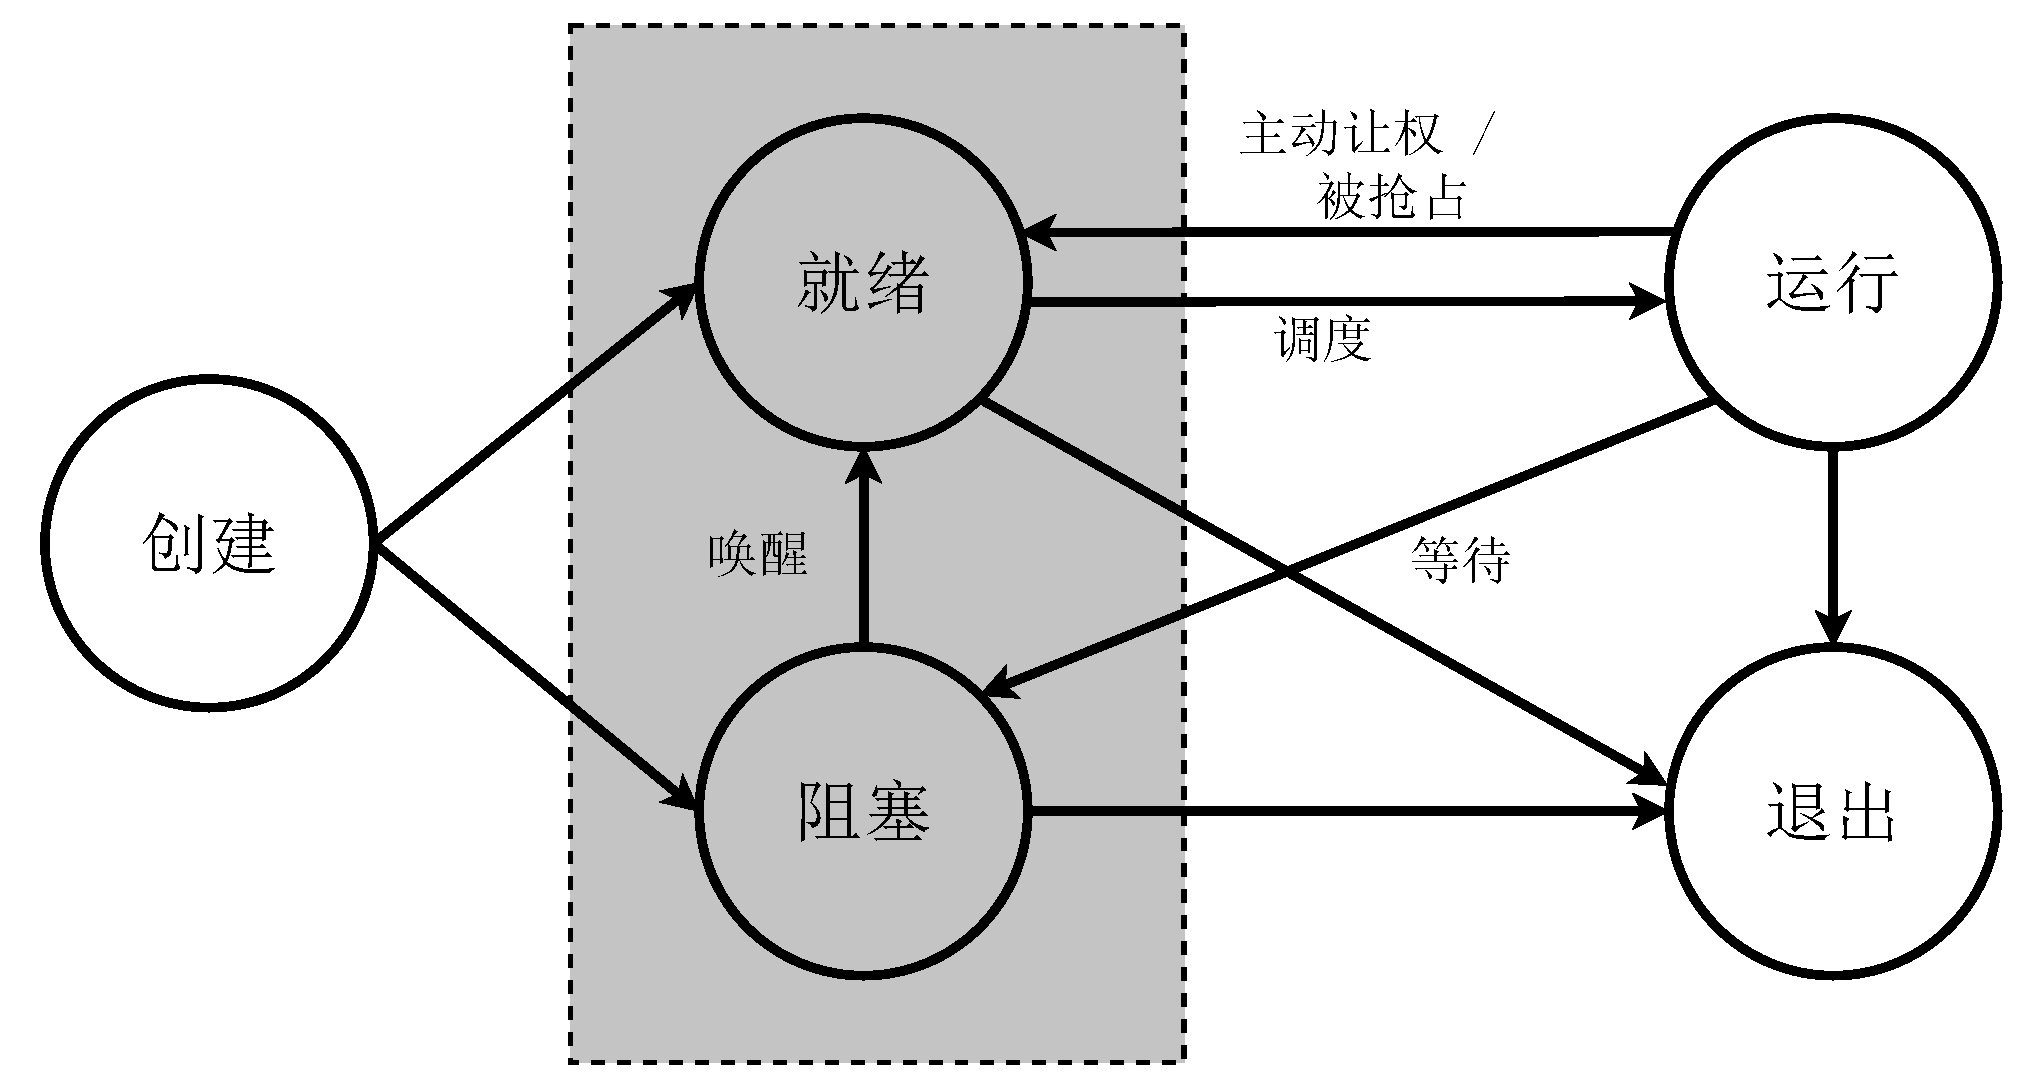
\includegraphics[width=0.8\textwidth]{figures/pdfs/task_state.pdf}
    \caption{基于软硬协同的任务状态模型}
    \label{figure:task_state}
\end{figure}

任务状态仍然为创建、就绪、运行、阻塞和退出这五种状态,其中灰色框线中的就绪态与阻塞态以及它们之间的状态转移由硬件任务调度器进行。硬件任务调度器在内部维护若干不同的就绪任务队列 $RQ_{*}$ 和阻塞任务队列 $BQ_{*}$,每个队列中存放任务的标识 $T_{(P_{i}, L_{j}, W_{k})}$(由任务的符号化标识 $T_{(P_{i}, L_{j}, S_{k})}$ 和任务的优先级 $W_{k}$ 等信息复合而成),并通过任务的优先级等信息维护任务队列的偏序关系。硬件调度器可以根据任务队列感知任务的状态以及优先级等信息,硬件通过将任务标识在这些队列中迁移实现对任务状态转移。硬件无法感知灰色框线外的其他任务状态,这些状态以及它们之间的转移由软件来维护,其他任务状态与就绪态、阻塞态之间的状态转移也由软件通过读写硬件调度器的响应端口来发起。任务的状态转移如下:

\begin{itemize}
    \item 创建 $\longrightarrow$ 就绪、创建 $\longrightarrow$ 阻塞:软件直接修改任务状态后,写硬件调度器的端口将创建的任务的标识添加至硬件调度器的就绪队列或者阻塞队列中;
    
    \item 就绪 $\longrightarrow$ 运行:软件读取硬件调度器的端口可以获取到就绪任务队列中最高优先级的任务标识,软件将任务的状态修改为运行态;
    
    \item 运行 $\longrightarrow$ 就绪:软件修改任务状态后,写硬件调度器的端口将任务标识添加至硬件调度器的就绪队列中;
    
    \item 运行 $\longrightarrow$ 阻塞:软件修改任务状态后,写硬件调度器的端口将任务标识添加至硬件调度器的阻塞队列中;
    
    \item 运行 $\longrightarrow$ 退出:软件直接修改任务状态;
    
    \item 阻塞 $\longrightarrow$ 就绪:硬件调度器根据特定的条件(例如收到中断信号)将阻塞队列中的任务标识添加至就绪队列中;这个过程硬件不直接修改任务状态,在软件从硬件调度器中取出就绪任务后,直接修改任务状态;
    
    \item 就绪 $\longrightarrow$ 退出、阻塞 $\longrightarrow$ 退出:软件向硬件调度器端口中写任务标识,硬件调度器将任务标识从就绪队列或阻塞队列中移除后,软件修改任务状态;
\end{itemize}

软件需要申请相应的就绪队列和阻塞队列,硬件任务调度器在成功分配了这些队列的硬件资源 $RQ_{(P_{i}, L{j})} + BQ_{(P_{i}, L{j})}$ 后,将会把这些队列相应的句柄(软件可以访问的硬件端口)返回给软件,软件通过该句柄来使用硬件任务调度器的功能。由于软件运行于一定的地址空间和特权级下(进程),在硬件队列申请成功后,直到进程生命周期结束或者软件主动释放掉硬件队列之前的这段时间,硬件队列与进程的地址空间 $P_{i}$ 和特权级 $L_{j}$ 相绑定。

使用硬件任务调度器,可以利用硬件机制来实现对任务队列的互斥访问,从而避免由于并发访问软件调度器带来的同步互斥开销。

\subsection{硬件中断处理机制}

\begin{figure}[htbp]
    \centering
    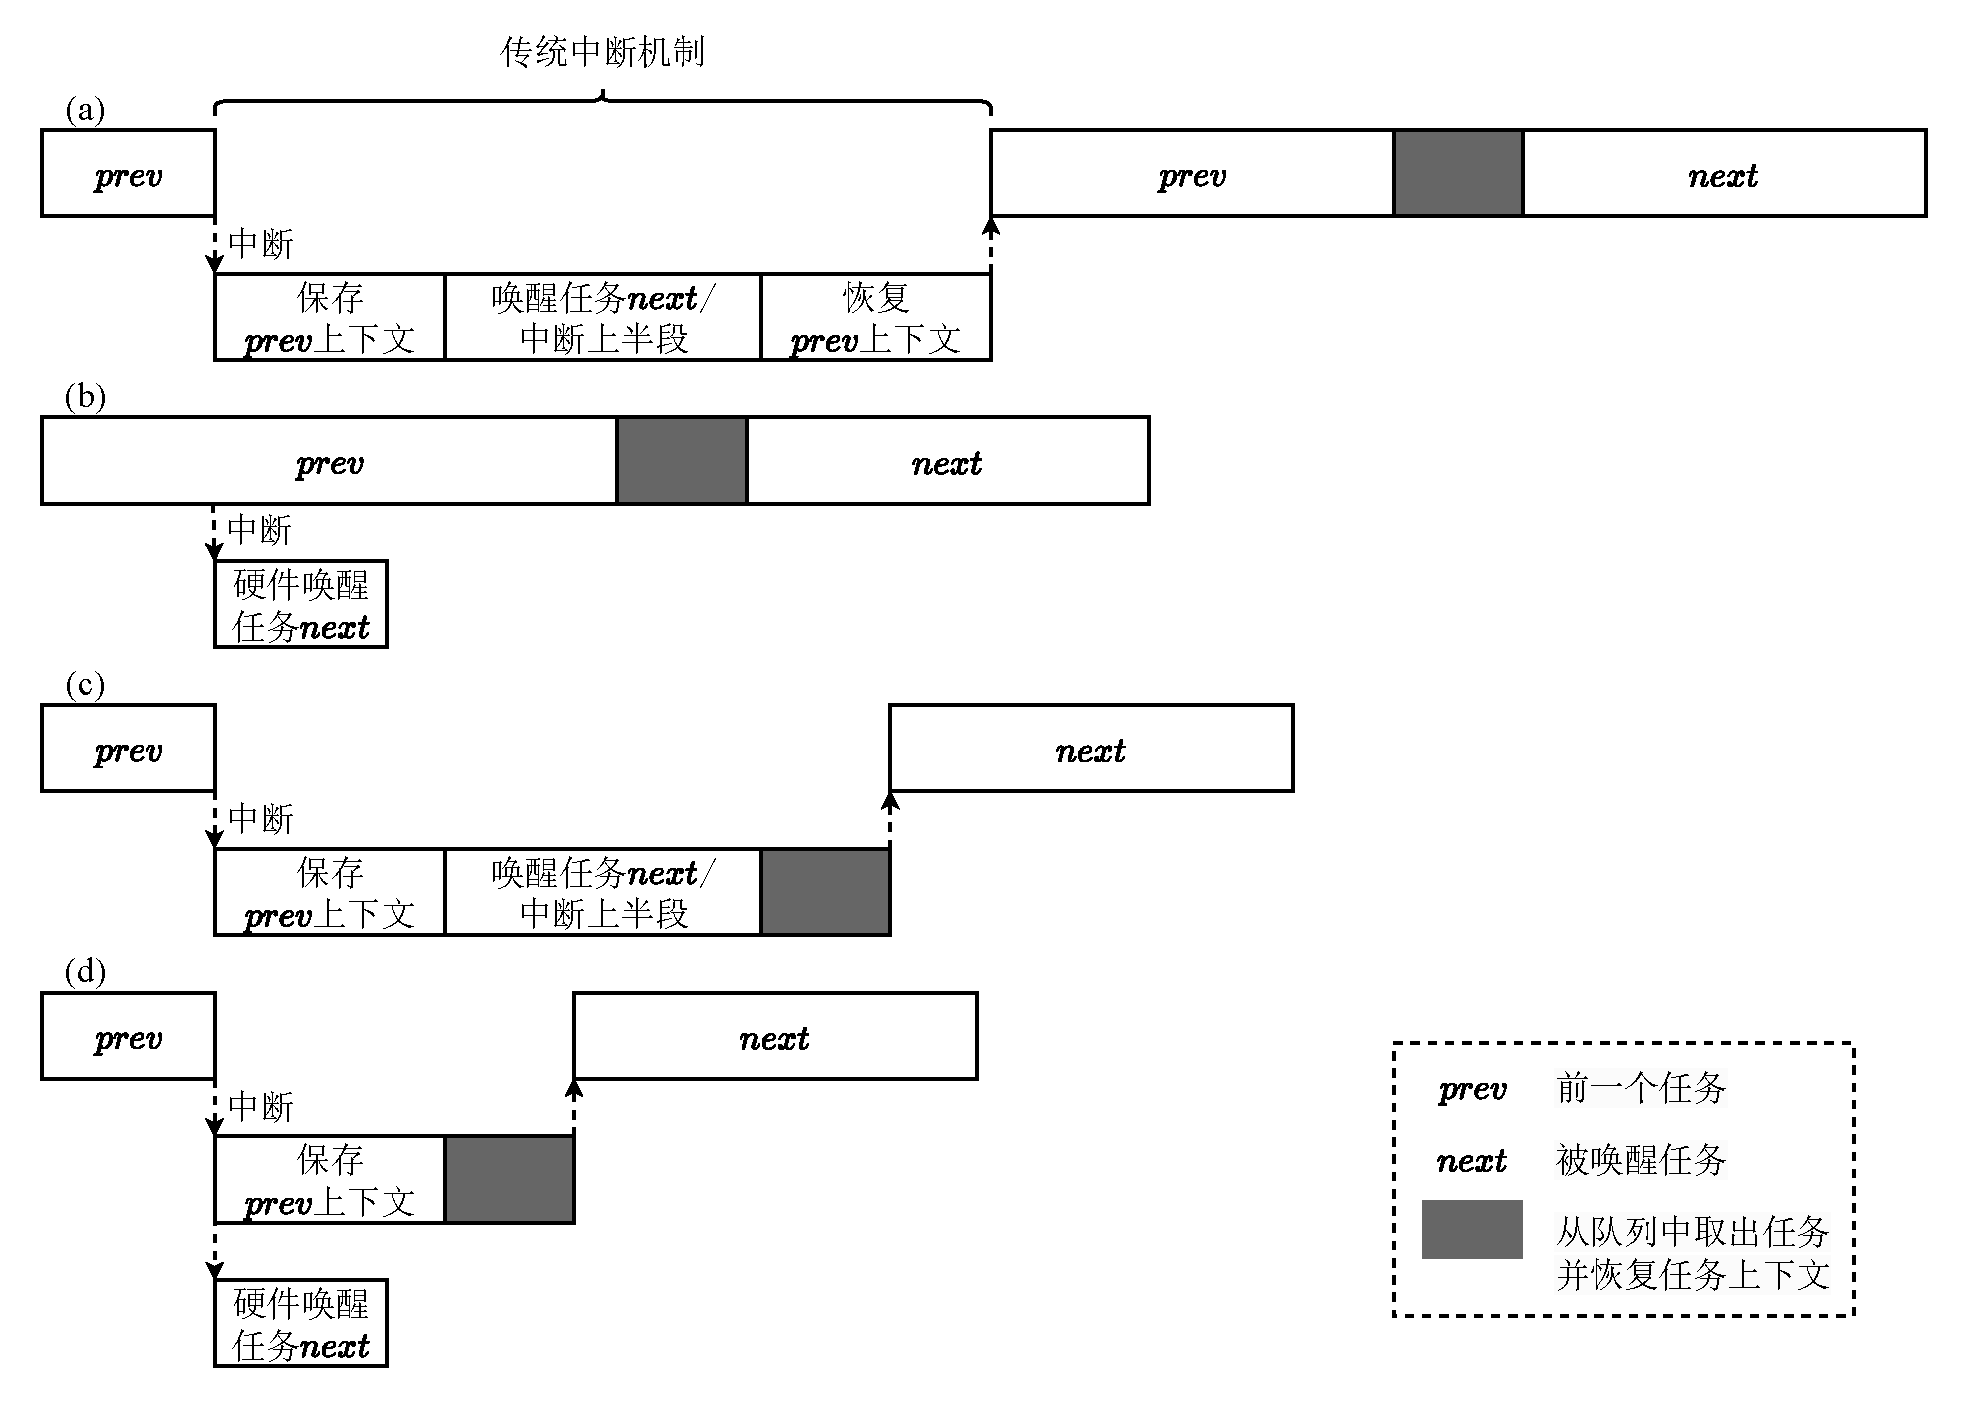
\includegraphics[width=\textwidth]{figures/pdfs/intr_demo.pdf}
    \caption{硬件处理中断图示,(a)为软件处理中断的流程,无任务抢占;(b)为硬件处理中断的流程,无任务抢占;(c)在(a)的基础上增加了任务抢占;(d)在(b)的基础上增加了任务抢占。}
    \label{figure:intr_demo}
\end{figure}

硬件中断处理机制的本质是用硬件电路来唤醒由于等待中断(I/O、定时器事件等)而进入阻塞状态的任务,这需要软硬件共同完成,其完整的流程如下:

\begin{enumerate}
    \item 软件向硬件调度器的端口中写任务标识,将其注册为某个中断信号的响应任务(硬件任务调度器将任务标识放入到与中断相关的阻塞队列中),预先将任务标识与中断进行绑定;
    \item 当硬件调度器收到中断信号后,根据中断信号的来源,找到对应的阻塞队列以及负责响应中断的任务标识,根据任务标识中的优先级信息,将任务标识从阻塞队列中移除,并放入到就绪队列中的合适位置;
    \item 如果唤醒的任务的优先级比当前正在 CPU 上运行的任务的优先级高,那么硬件任务调度器应该向 CPU 发送中断,CPU 在收到硬件任务调度器的中断信号后,直接进行任务切换。
\end{enumerate}

% \begin{figure}[htbp]
%     \centering
%     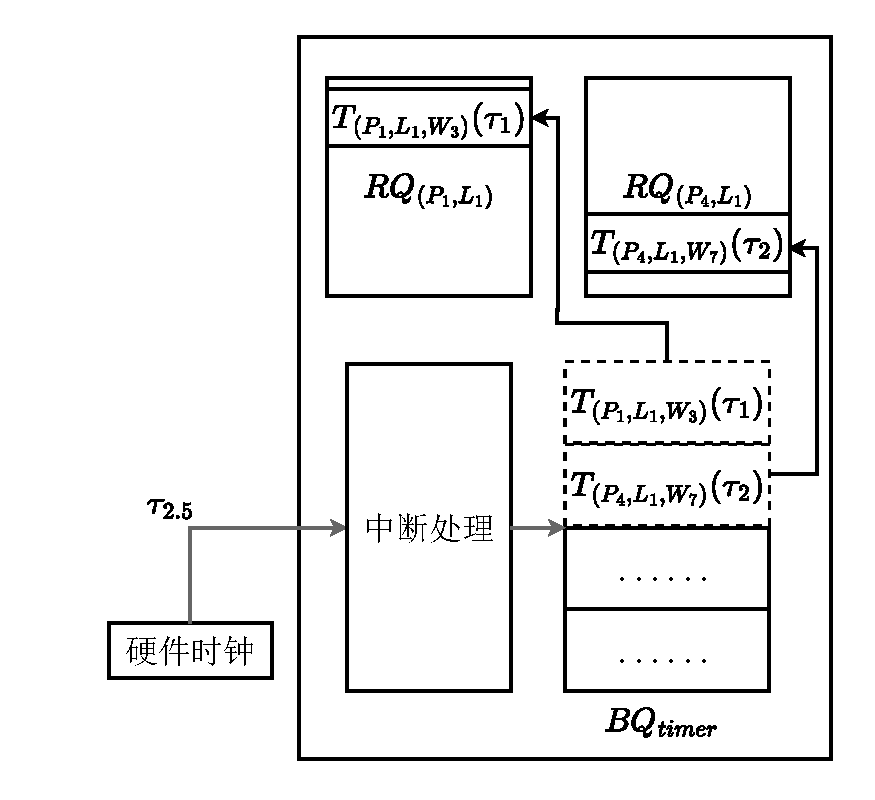
\includegraphics[width=0.8\textwidth]{figures/pdfs/timer.pdf}
%     \caption{硬件处理时钟中断}
%     \label{figure:timer}
% \end{figure}

% 以硬件处理时钟中断为例(如图 \ref{figure:timer}),硬件任务调度器在内部实现了与时钟中断相关的阻塞任务队列($BQ_{timer}$)来维护由于等待定时器事件而进入阻塞状态的任务标识($T_{(P_{i}, L_{j}, W_{k})}(\tau_{t})$,标识中增加了定时器的截止时间 $\tau_{t}$),该队列根据任务所等待的定时器的截止时间 $\tau_{t}$ 的先后顺序进行排序。在 $\tau_{2.5}$ 时刻,硬件时钟产生时钟中断,将信号发送给硬件任务调度器,硬件任务调度器检查 $BQ_{timer}$ 队列头部的任务所等待的定时器事件的截止时间,发现任务标识 $T_{(P_{1}, L_{1}, W_{3})}(\tau_{1})$ 和 $T_{(P_{4}, L_{1}, W_{7})}(\tau_{2})$ 的截止时间小于当前时间,因此,硬件任务调度器根据任务标识中的进程标识和特权级标识找到对应的就绪队列,并根据任务标识中的优先级信息将其放入到就绪队列的适当位置,完成硬件中断处理。

通过硬件快速响应中断,唤醒阻塞的任务,可以让 CPU 不被一些中断信号打断,减少由于中断导致的中断上下文切换开销。若被唤醒的任务优先级较高,需要进行任务切换,在这种情况下,仍然可以减少由于中断导致的调度开销,硬件中断处理机制与传统机制的对比如图 \ref{figure:intr_demo} 所示。

\subsection{硬件支持的任务通信机制}

通信中的两个任务分别为发送方与接收方,它们属于不同的地址空间或不同特权级下的进程。使用硬件支持的任务通信机制的前提是通信的双方都使用了硬件提供的任务调度器功能(双方进程分别使用不同的任务队列),并且,在上述的硬件中断处理机制的基础上,将中断信号的发送方从硬件设备扩展为软件上的发送方任务。此外,硬件中还需要维护与双方通信能力相关的能力槽,并配置额外的能力检查机制来避免恶意通信。其完整的通信流程如下:

\begin{enumerate}
    \item 发送方与接收方申请使用硬件任务调度器;

    \item 发送方任务向硬件任务调度器的端口中写接收方任务的进程标识以及中断号,硬件任务调度器将这两项信息填写至发送方的发送能力槽中,从而注册可以向指定接收方进程发送的指定中断的能力;
    
    \item 接收方任务向硬件任务调度器的端口中写发送方任务的进程标识、中断号以及自己的标识,硬件任务调度器将这些信息填写至接收方的接收能力槽中,从而注册可以接收指定发送方的指定中断的能力;
    
    \item 发送方任务向硬件任务调度器的端口中写接收方的进程标识以及中断号,尝试进行通信。硬件任务调度器首先检查发送方的发送能力槽中是否存在对应的接收方进程标识以及中断号。如果存在,则硬件任务调度器根据接收方的进程标识找到对应的接收方进程所使用的就绪队列以及接收能力槽,如果接收能力槽中存在对应的发送方的进程标识、中断号以及接收方的任务标识,则硬件任务调度器将接收方的任务标识放入到接收方的就绪队列中的适当位置,完成通信。

\end{enumerate}

基于硬件支持的通信机制,跨域不同地址空间和特权级的执行流之间可以实现快速交互,减少了切换地址空间以及特权级的开销,图展示了信号机制与使用 TAIC 机制进行通信的对比。

\begin{figure}
    \centering
    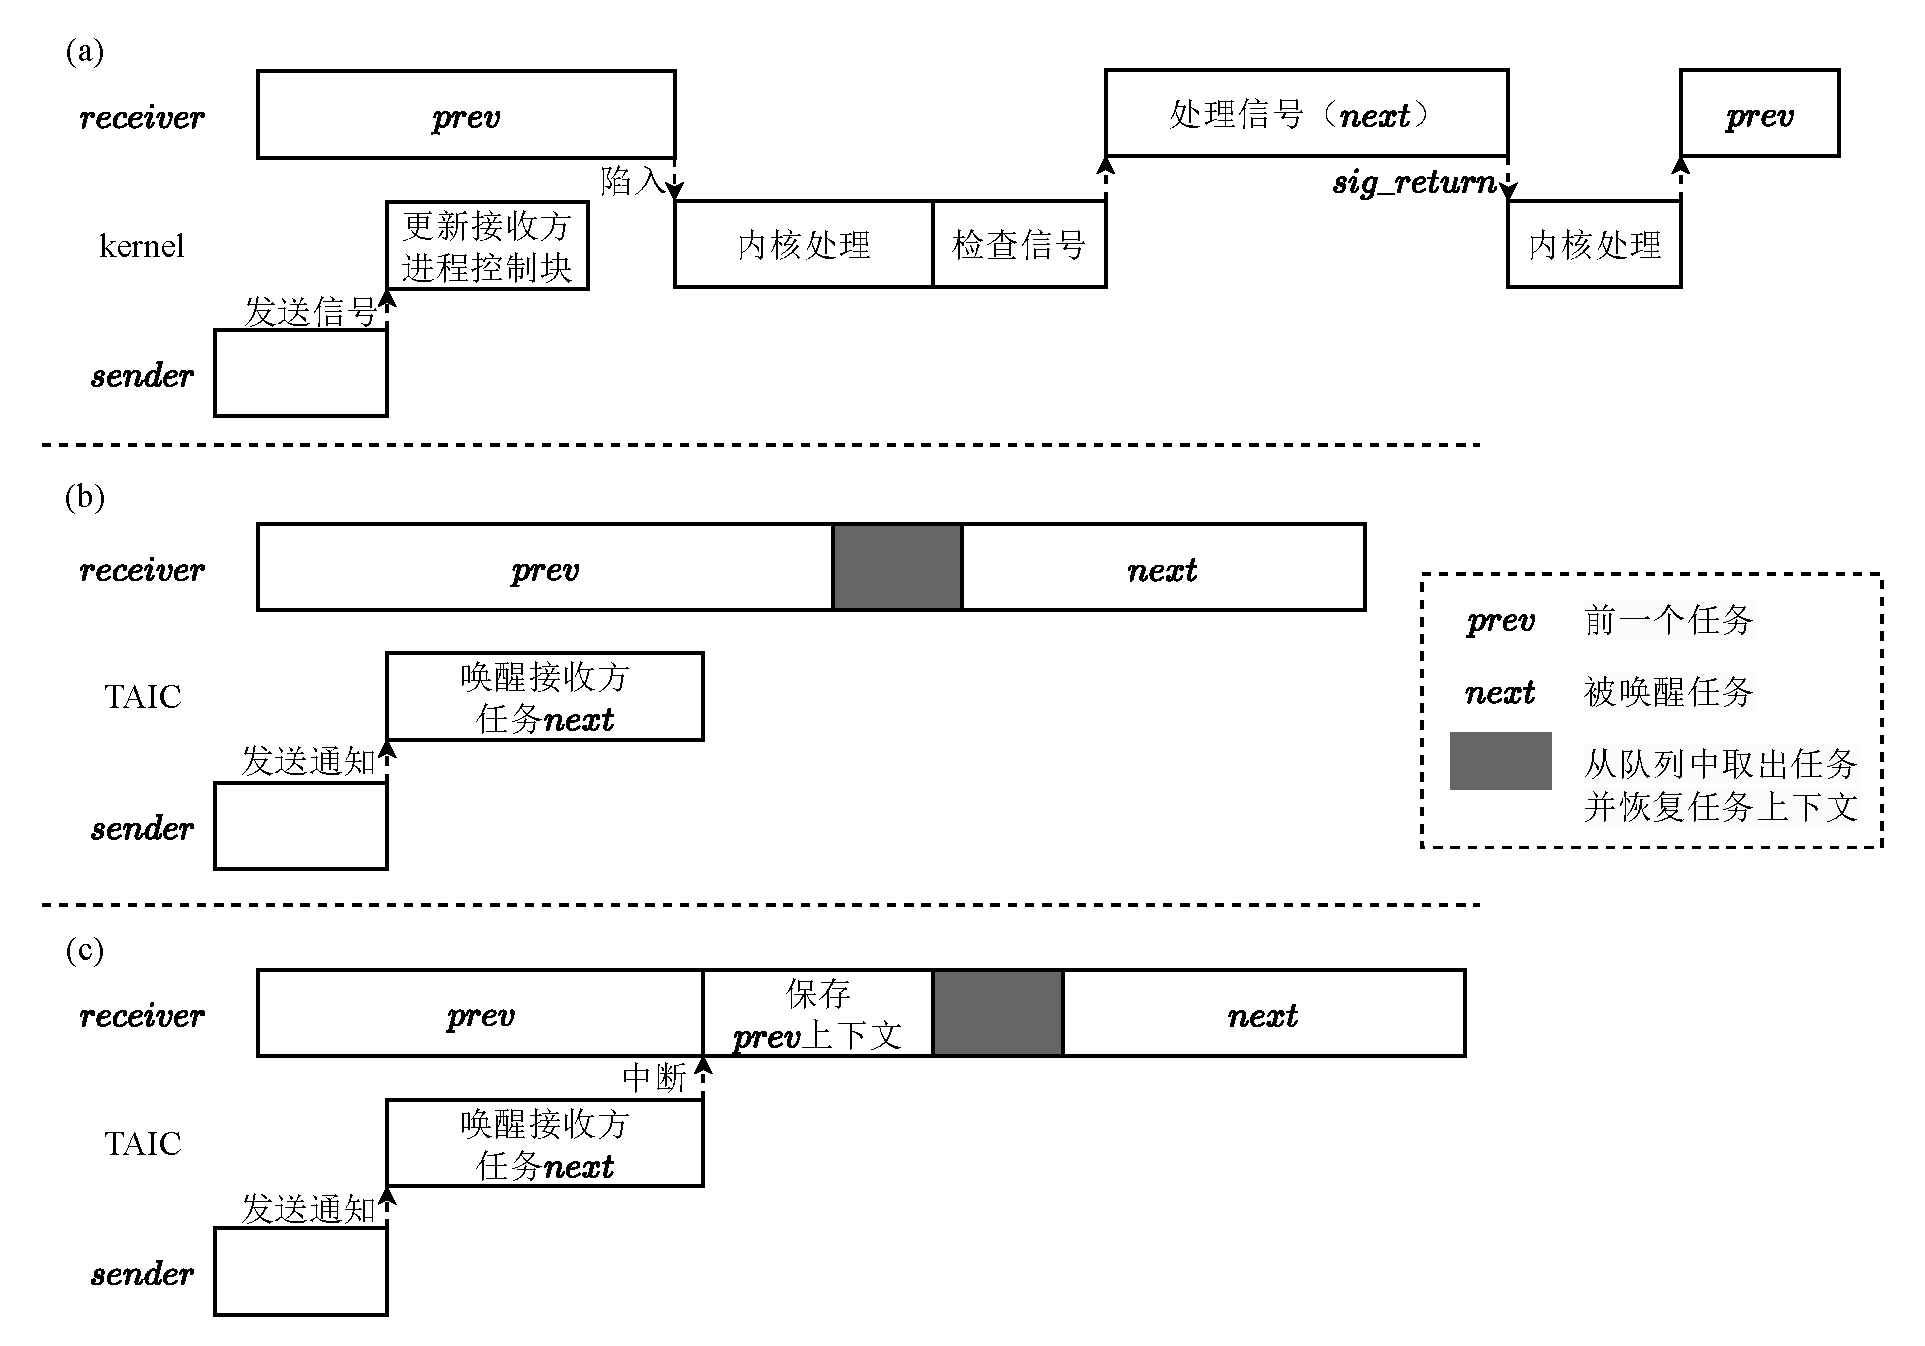
\includegraphics[width=\textwidth]{figures/pdfs/communicate_demo.pdf}
    \caption{IPC 对比,(a)为基于信号机制的通信流程;(b)为使用 TAIC 机制的通信流程,没有任务抢占;(c)在(b)的基础上增加了任务抢占。}
\end{figure}

\section{软硬件交互接口}

I/O 端口作为软件访问硬件的入口,也是硬件响应软件操作并返回结果的媒介。软件通过向 I/O 端口发送读写命令,将数据与控制信号传递给硬件,最终转化为对硬件中的寄存器或状态的操作,从而驱动硬件完成特定的功能。在本文的基于软硬协同的中断响应和任务调度机制中,软硬件相互协作,共同完成任务调度、中断处理以及任务通信等功能,软硬件之间的交互接口如表 \ref{table:io_interface} 所示。

\begin{table}[htbp]
    \centering
    \caption{软硬件交互接口}
    \label{table:io_interface}
    \begin{tabular}{lll}
        \toprule
        功能 & 接口 & 说明 \\
        \midrule
        \multirow{2}{*}{\makecell[l]{硬件资源 \\ 申请与回收}} & alloc & \makecell[l]{软件写端口,申请的队列资源,并从端口中读出 \\ 队列资源句柄} \\
        & free & \makecell[l]{软件写需要回收的句柄,硬件回收队列资源} \\ \hline
        \multirow{3}{*}{任务调度} & task\_enqueue & \makecell[l]{软件写任务标识,硬件将标识添加至就绪队列中} \\
        & task\_dequeue & \makecell[l]{软件从硬件中读出优先级最高的就绪任务标识} \\
        & remove\_task & \makecell[l]{软件写任务标识,硬件将删除队列中的任务标识} \\ \hline
        \multirow{2}{*}{外部中断处理} & register\_extint & \makecell[l]{软件写任务标识,将任务与中断绑定} \\
        & unregister\_extint & \makecell[l]{软件取消任务与中断之间的绑定} \\ \hline
        \multirow{5}{*}{任务通信} & register\_sender & \makecell[l]{软件写接收方进程标识和中断号,注册发送能力} \\
        & unregister\_sender & \makecell[l]{软件写接收方进程标识和中断号,取消发送能力} \\
        & register\_receiver & \makecell[l]{软件写发送方进程标识、中断号和接收方任务 \\ 标识,注册接收能力} \\
        & unregister\_receiver & \makecell[l]{软件写发送方进程标识和中断号,取消接收能力} \\
        & send & \makecell[l]{软件写接收方进程标识和中断号,发起通信} \\
        \bottomrule
    \end{tabular}
\end{table}

\section{本章小结}

本章提出基于执行流的任务模型,从“\textbf{任务通信}”的视角出发,将任务调度、中断处理以及任务通信组合成统一整体,利用硬件快速、高效等特点对其进行加速,设计了基于软硬协同的中断响应和任务调度机制,综合性地减小系统开销,提高系统应对应用场景复杂多样的性能需求。

\chapter{基于软硬协同的中断响应和任务调度实现}

本章根据第三章所述的任务模型和设计方案,在 FPGA 平台上实现了上述的具备中断处理、任务通信以及任务调度的控制器(TAIC,Task Aware Interrupt Controller),并且进行了相关的软件适配,实现了基于软硬协同的中断响应和任务调度机制的系统原型。

\section{系统整体结构}

图 \ref{figure:arch} 给出了基于软硬协同的中断响应和任务调度系统的整体架构。系统由 CPU、TAIC 和外部设备三部分组成。外部设备的中断信号连接到 TAIC 的中断处理模块中,TAIC 内部维护了若干套用于不同的地址空间和特权级下的队列资源(包括就绪队列、外部中断能力槽、接收能力槽和发送能力槽),不同的队列资源之间通过任务通信模块构建硬件的通信通道。CPU、TAIC 与外部设备通过总线相连。运行于 CPU 上的处于不同地址空间和特权级之间的任务通过软硬件交互接口使用 TAIC 提供的中断处理、任务调度和任务通信功能。

\begin{figure}[htbp]
  \centering
  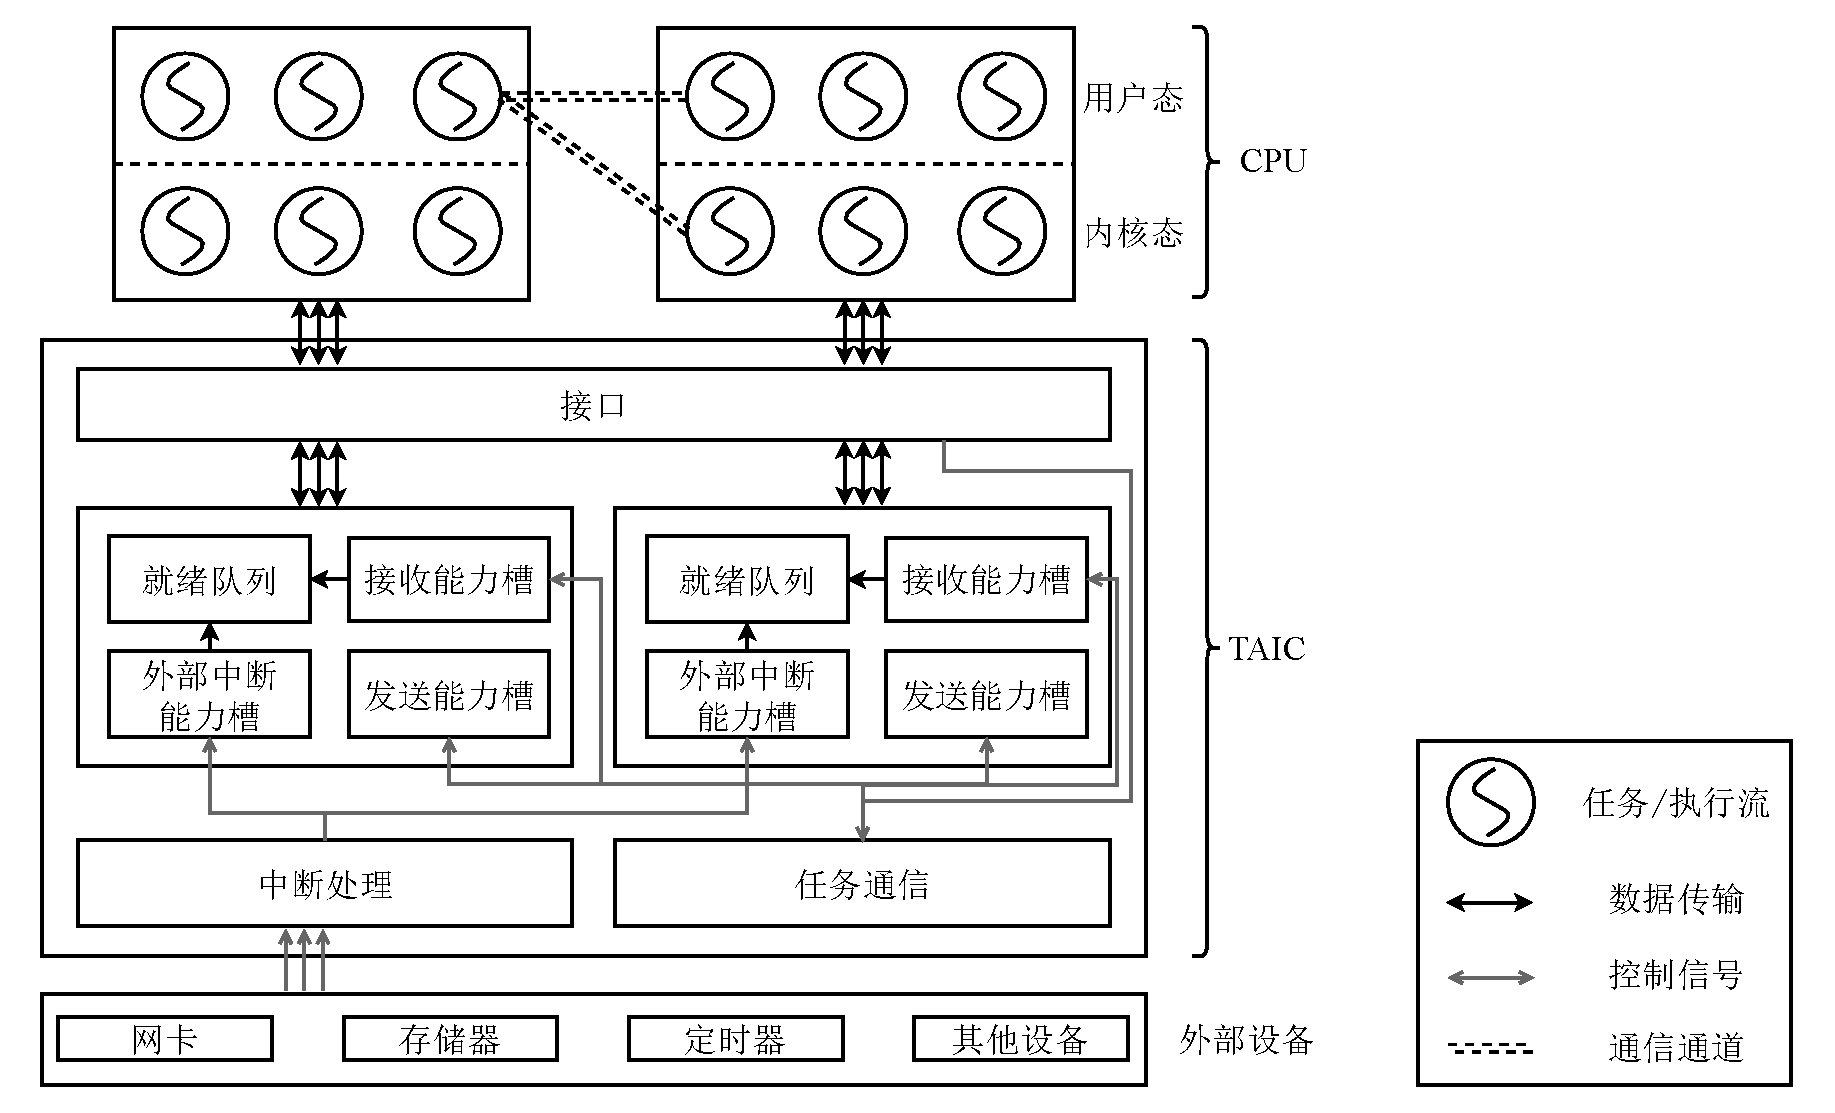
\includegraphics[width=0.8\textwidth]{figures/pdfs/arch.pdf}
  \caption{基于软硬协同的中断响应和任务调度系统整体架构}
  \label{figure:arch}
\end{figure}

\section{控制器实现}

根据 TAIC 提供的功能划分,TAIC 由四个模块构成:任务调度、中断处理、任务通信和队列资源分配与回收。

\subsection{任务调度}

TAIC 内部维护了若干任务队列,并且 TAIC 能够在不同的任务队列之间迁移任务标识,维持任务队列的偏序关系,以此来向软件提供任务调度的功能。

其中就绪队列的实现直接在硬件层面提供了软件中的任务队列所需要的出队、入队、优先级排序和负载均衡等功能,能够满足软件的任务调度需求。就绪队列由一块脉冲阵列和若干个局部队列元信息组成,如图 \ref{figure:ready_queue} 所示。

\begin{figure}
  \centering
  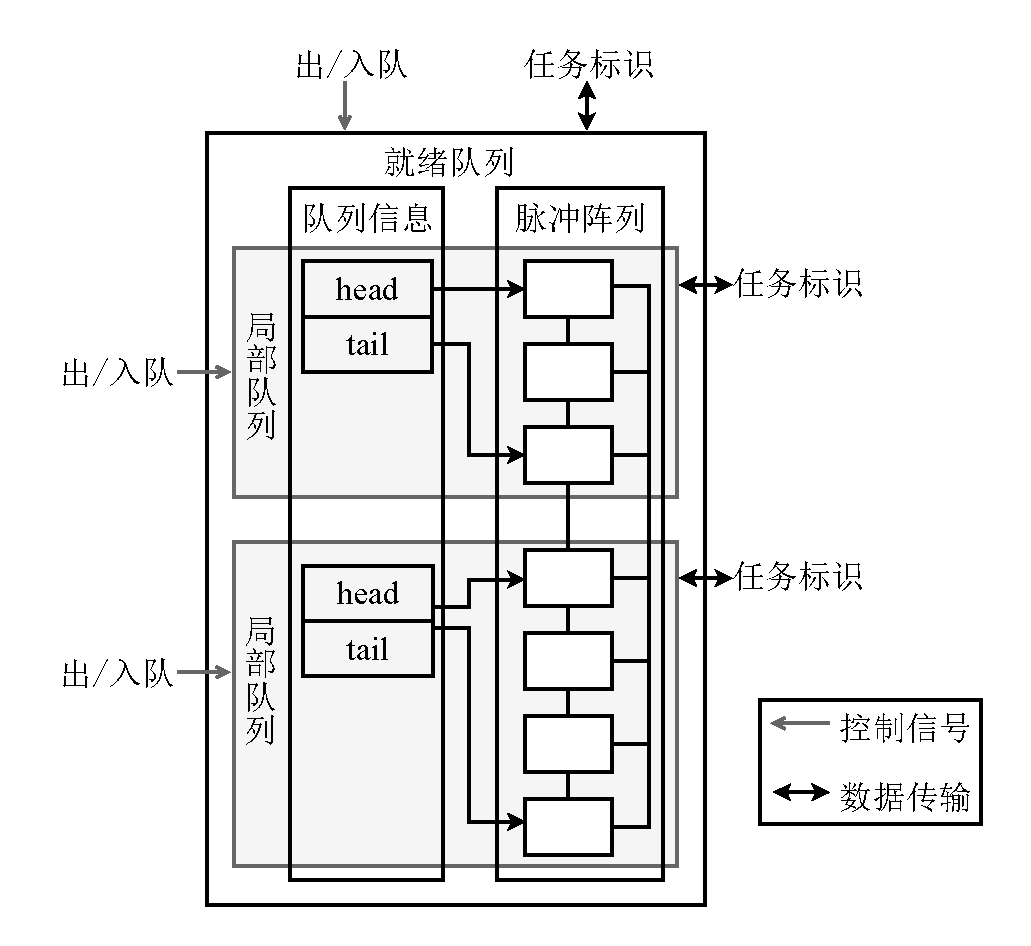
\includegraphics[width=\textwidth]{figures/pdfs/ready_queue.pdf}
  \caption{就绪队列}
  \label{figure:ready_queue}
\end{figure}

脉冲阵列用于存放任务标识,当需要删除某个位置的任务标识时,该位置后的所有任务标识自动前移即可完成删除操作;当需要在某个位置插入任务标识时,先将该位置包括后续的所有任务标识后移,然后再将任务标识插入到该位置即可完成插入操作。

基于脉冲阵列,只需要记录队列在脉冲阵列中的头部 $head$ 和尾部 $tail$ 位置即可实现局部队列。由于局部队列共用同一块脉冲阵列,因此当某个局部队列在进行出/入队操作时,位于该局部队列后的所有局部队列的 $head$ 和 $tail$ 指针都需要更新。局部队列支持的操作为:

\begin{itemize}
  \item 出队:取出脉冲阵列中 $head$ 处的任务标识,将自己的 $tail$ 指针 -1,将后续所有局部队列的 $head$ 和 $tail$ 指针 -1;
  \item 入队:将任务标识插入到脉冲阵列中 $tail$ 处,将自己的 $tail$ 指针 +1,将后续所有局部队列的 $head$ 和 $tail$ 指针 +1;
\end{itemize}

这些局部队列共同组成了一个就绪队列(全局队列),既可以单独对局部队列执行出/入队操作,也可以对全局队列执行出/入队操作。全局队列的容量存在上限(脉冲阵列可以存放的任务标识的数量),但局部队列的容量没有固定上限,当全局队列达到容量上限时,对任意局部队列进行的入队操作将会失败,无法插入任务标识。局部队列在执行出队操作时集成了负载均衡的功能,当某个局部队列为空时,会从其他具有任务的局部队列中窃取任务标识(窃取的顺序为局部队列的 $head$ 指针指向的脉冲阵列位置的顺序);只有当整个全局队列为空时,才会返回空值。

基于局部队列的窃取机制以及窃取的顺序,整个全局队列可以当作优先级队列使用,其中每个局部队列中存放优先级相同的任务标识,并且按照先进先出的规则进行排序。不同的局部队列的优先级不同,$head$ 指针在脉冲阵列的位置越靠前,优先级越高。

基于上述的就绪队列实现,软件可以灵活地使用局部队列和全局队列,已实现不同的调度策略,并且减少因为固定局部队列容量导致的硬件资源的浪费。

由于硬件资源有限,阻塞队列只用于保存因为等待外部设备以及等待任务通信而进入阻塞状态的任务的标识,对应的实现为外部中断能力槽和接收能力槽,分别在 \ref{section:interrupt} 和 \ref{section:communication} 中描述。

\subsection{中断处理}
\label{section:interrupt}

TAIC 快速处理中断机制依赖于任务队列中的维护的外部中断能力槽,它记录了由于等待外部设备中断而进入阻塞状态的任务的标识。由于应用程序通常只有一个任务用于处理外部中断,因此,针对每个外部中断信号只准备了一个槽位。其结构以及处理流程如图 \ref{figure:extintr} 所示。

\begin{figure}[htbp]
  \centering
  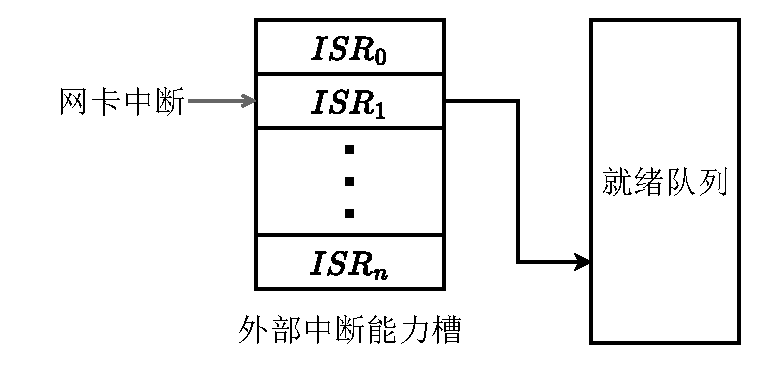
\includegraphics[width=0.8\textwidth]{figures/pdfs/extintr.pdf}
  \caption{外部中断处理}
  \label{figure:extintr}
\end{figure}

$ISR_{i}$ 表示与中断号为 $i$ 相关的任务标识,在使用硬件快速处理中断能力时,需要软件向外部中断能力槽中注册任务标识(该任务为阻塞状态),注册成功即为使能了硬件外部中断处理机制。当外部设备产生中断信号时,TAIC 的中断处理模块会根据中断信号来检查对应的槽位,若其中存在任务标识,将任务标识从槽中取出,并放入到就绪队列中的合适位置,以此来唤醒因为等待外部设备中断而进入阻塞状态的任务。一旦完成唤醒操作,外部中断能力槽中该中断对应的槽位会被清空,TAIC 的快速处理该中断的能力会被屏蔽,直到软件再次注册该中断的处理任务重新使能该机制。

此外,若中断的处理任务的优先级较高,TAIC 会向 CPU 发送中断信号,CPU 在收到中断信号后,直接进行任务切换。TAIC 的硬件快速处理中断机制可以无视特权级,可以在用户态使用,但需要额外的机制来保证任意时刻只有一个进程或内核在使用同一个外部设备。但对于某些特殊的应用场景,例如在虚拟化场景中,多个内核使用同一个硬件定时器,则可以通过 TAIC 来实现时钟设备的虚拟化。

\subsection{任务通信}
\label{section:communication}

由于任务通信的发送方和接收方是处于不同地址空间和特权级下的任务,而进程可以用于区分地址空间和特权级,且进程属于操作系统,因此使用操作系统标识和进程标识来表示任务所出的环境。因此,TAIC 基于操作系统标识和进程标识,在内部维护了若干的发送能力槽和接收能力槽,用于构建硬件支持的跨越不同环境的任务通信通道。

发送能力槽中记录了当前环境下,可以向哪些接收方 $(recv\_os_{i}, recv\_proc_{j})$ 发起通信以及通信通道的编号$irq_{k}$,而接收能力槽则记录了当前环境下能够接收哪些发送方 $(send\_os_{l}, send\_proc_{m})$的通信请求、通信通道编号 $irq_{n}$,并且记录了当前环境下因为等待任务通信而进入阻塞状态的任务标识 $isr_{x}$。发送能力槽和接收能力槽的结构以及任务通信流程如图 \ref{figure:communication} 所示。

\begin{figure}[htbp]
  \centering
  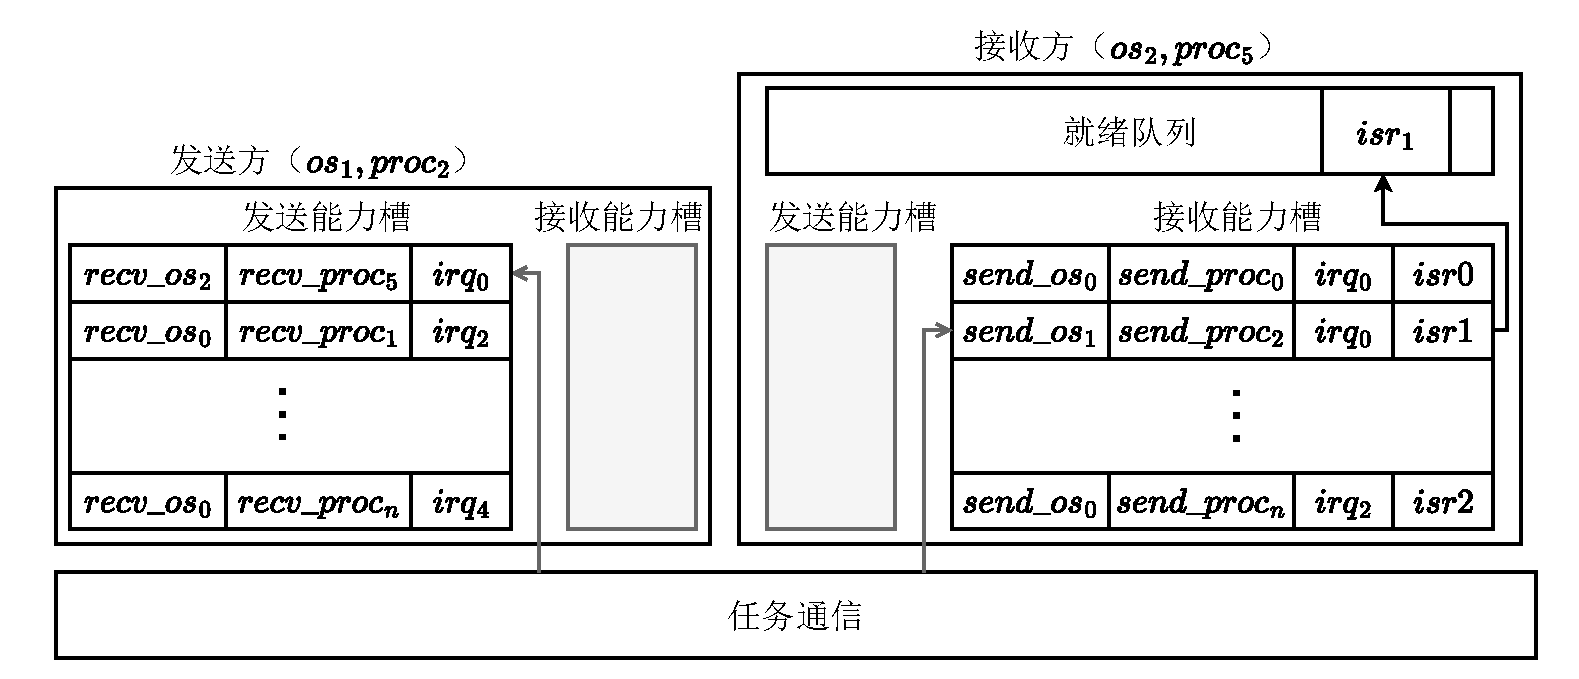
\includegraphics[width=\textwidth]{figures/pdfs/communication.pdf}
  \caption{任务通信}
  \label{figure:communication}
\end{figure}

在使用硬件支持的任务通信能力时,发送方需要向发送能力槽中写入接收方的操作系统标识和进程标识,以及通信通道的编号,注册成功即为使能了发送能力。接收方需要向接收能力槽中写入发送方的操作系统标识和进程标识、通信通道的编号以及任务标识,注册成功即为使能了接收能力。

发送方通过向 TAIC 的端口中写入接收方的操作系统标识、进程标识以及通信通道编号来发起通信,TAIC 的任务通信模块根据发送方提供的标识信息,首先检查发送方的发送能力槽中是否存在对应的条目,如果不存在,则通信失败;若存在条目,任务通信模块根据发送能力槽条目中记录的接收方的操作系统标识、进程标识以及通信通道标识,检查接收方的接收能力槽中是否存在对应的条目,如果不存在,则通信失败;如果存在,任务通信模块将接收能力槽中对应的条目清除,将等待通信的任务标识放入到就绪队列中的合适位置,完成任务通信。若唤醒的接收方任务的优先级较高,TAIC 会向 CPU 发送中断信号,CPU 在收到中断信号后,直接进行任务切换。

\subsection{资源分配与回收}

每套资源由就绪队列、外部中断能力槽、发送能力槽和接收能力槽组成,向位于特定地址空间和特权级下的软件提供任务调度、中断处理和任务通信功能。由于操作系统与进程可以用于区分地址空间和特权级,因此本文使用操作系统和进程的标识符 $(os\_id, proc\_id)$ 来区分不同的资源,软件要使用这些功能时,需要向 TAIC 的资源分配接口写入操作系统标识和进程标识,TAIC 会根据这些标识符来分配相应的资源,最终返回软件可以操作的句柄。资源分配的流程如下:

\begin{enumerate}
  \item 向 TAIC 的资源分配接口依次写入 $os\_id$ 和 $proc\_id$。
  
  \item TAIC 根据 $os\_id$ 和 $proc\_id$ 查找是否已经分配了对应的资源,若没有,则分配一套资源,将其标记为 $(os\_id, proc\_id)$ 已使用,并在资源初始化之后执行 \ref{item:alloc_handle};若已经分配,则执行 \ref{item:alloc_handle};如果控制器中没有空闲资源,则分配失败。
  
  \item \label{item:alloc_handle} 分配软件操作句柄,句柄包括了对这套资源中的就绪队列中的某个局部队列、外部中断能力槽、发送能力槽和接收能力槽的操作接口。
\end{enumerate}

在相同的地址空间和特权级 $(os\_id, proc\_id)$ 中,不同的句柄对中断处理、任务通信等接口的操作是等价的,都会对外部中断能力槽、发送能力槽和接收能力槽产生相同的影响,但对就绪队列中的局部队列的操作是不同的,这是为了保证软件在使用这些接口时是一致的。

资源回收的流程如下:

\begin{enumerate}
  \item 向 TAIC 的资源回收接口依次写入 $os\_id$ 和 $proc\_id$。
  
  \item TAIC 根据 $os\_id$ 和 $proc\_id$ 查找是否已经分配了对应的资源,若没有,则回收失败;若已经分配,则执行 \ref{item:free_handle}。
  
  \item \label{item:free_handle} 回收软件操作句柄,释放软件对该句柄对应的局部队列的操作权限。若这套资源所有申请的操作句柄都被回收时,将资源标记为未使用。
\end{enumerate}

\section{任务抢占}

TAIC 提供了中断处理和任务通信的能力,硬件直接唤醒了对应的阻塞任务,但这不意味着被唤醒的任务会马上执行,若 CPU 上正存在其他的任务执行,而被唤醒的任务优先级较高,则会导致被唤醒任务的响应延时增加。因此,TAIC 会在被唤醒的任务优先级较高时,向 CPU 发送中断,实现了抢占式任务调度。由于被唤醒的任务可能处于内核态或用户态,因此 TAIC 根据被唤醒的任务标识中的操作系统标识和进程标识来判断任务所处的特权级,向 CPU 发送不同的中断信号。因此需要实现用户态中断扩展。本文在 rocket-chip 软核 \cite{rocket-chip} 上增加了用户态中断相关的控制寄存器以及 $uret$ 指令,并且将 TAIC 的中断信号与 CPU 的 $mip$ 寄存器的 $SSIP$ 和 $USIP$ 位相连,实现了 RISC-V 的 N 扩展。

当被唤醒的任务处于内核态且优先级较高时,TAIC 会产生中断信号,将 $mip$ 寄存器的 $SSIP$ 位拉高,CPU 跳转至内核态的中断向量寄存器 $stvec$ 指向的位置,保存被打断任务的寄存器现场,从 TAIC 中取出被唤醒的任务标识并执行任务,从而减少响应延时。

当被唤醒的任务处于用户态,这里的处理比唤醒处于内核态的任务更加复杂。可以分为两类:

\begin{enumerate}
  \item \label{item:uintr_online} 当 CPU 正在运行与被唤醒任务处于相同进程和特权级下的其他任务,若被唤醒任务的优先级较高,则 TAIC 会产生中断信号,将 $mip$ 寄存器的 $USIP$ 位拉高,CPU 跳转至用户态的中断向量寄存器 $utvec$ 指向的位置,保存被打断任务的寄存器现场,从 TAIC 中取出被唤醒的任务标识并执行任务,从而减少响应延时。
  \item 若当前 CPU 正在执行其他的与被唤醒任务处于不同地址空间或不同特权级的任务时,TAIC 会暂时挂起这次唤醒所产生的中断,直到 CPU 再次回到 \ref{item:uintr_online} 这种情况。
\end{enumerate}

\begin{figure}[htbp]
  \centering
  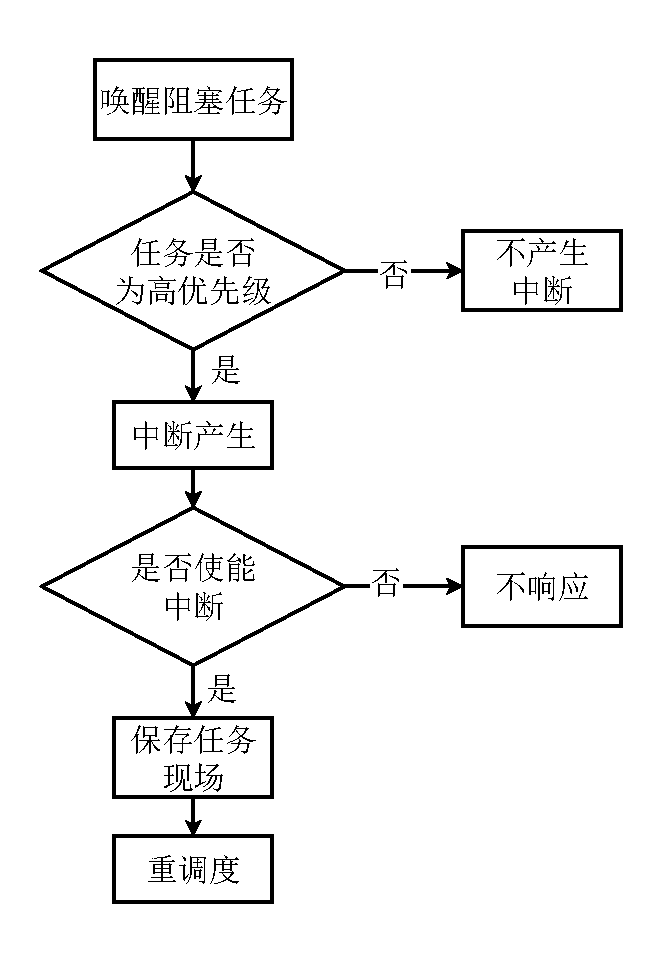
\includegraphics[width=0.6\textwidth]{figures/pdfs/userintr.pdf}
  \caption{任务抢占的流程}
  \label{figure:userintr}
\end{figure}

\section{软件适配}

TAIC 可以与现有的进程、线程或协程任务模型进行结合,线程与协程模型建立在进程提供的地址空间隔离机制上,将 TAIC 的端口映射到各自的地址空间中,即可向 TAIC 申请硬件资源用于任务调度、中断处理和任务通信。软件与 TAIC 的交互通过申请获取的硬件资源句柄进行。

\subsection{申请硬件资源}

TAIC 中的硬件资源通过操作系统标识和进程标识进行区分,因此在申请使用 TAIC 的硬件资源时,需要向资源分配端口写操作系统标识 $os\_id$ 和进程标识 $pid$。在内核中使用 TAIC 时,$os\_id$ 为一个固定的数值 $OSID$(由内核在初始化时进行约定),$pid$ 为 0,因此,内核向 TAIC的资源分配接口写入 $(OSID, 0)$ 即可使用 TAIC 提供的功能。在用户态使用时,则需要通过 \verb|get_taic_handle| 系统调用,该系统调用首先向 TAIC 的资源分配端口写入 $(OSID, pid)$ 申请资源句柄,并将资源句柄对应的端口映射到用户进程的地址空间中,最终将资源句柄返回给用户态,对应的伪代码为 \ref{alg:get_taic_handler}。

\floatname{algorithm}{系统调用}
\begin{algorithm}
  \caption{get\_taic\_handler}
  \label{alg:get_taic_handler}
  \begin{algorithmic}[1]
    \Require
    \Ensure handler
    
    \State  pid \gets get\_pid()
    \State  osid \gets OSID
    \State  taic\_base \gets TAIC\_BASE
    \State  size \gets HANDLER\_SIZE
    \State  handler\_id \gets taic\_alloc(osid, pid) {\Comment{申请 TAIC 资源,获取资源编号}}
    \If {handler\_id = $0$}
        \State  handler \gets $-1$
        \Return handler
    \EndIf
    \State handler\_addr \gets handler\_addr(handler\_id, 
    \Statex \qquad \qquad \qquad \qquad \qquad \qquad taic\_base) {\Comment{根据 TAIC 基址和资源编号,获取资源基址}}
    \State mem\_fd \gets open(\textquotedbl/dev/mem\textquotedbl, O\_RDWR)

    \If {mem\_fd = $-1$}
        \State taic\_free(handler\_id)
        \State handler \gets $-1$
        \Return handler
    \EndIf
    \State handler \gets mmap(NULL, size, 
    \Statex \qquad \qquad \qquad \qquad PROT\_READ | PROT\_WRITE, 
    \Statex \qquad \qquad \qquad \qquad MAP\_SHARED, 
    \Statex \qquad \qquad \qquad \qquad mem\_fd, handler\_addr) {\Comment{将 TAIC 资源句柄映射到进程地址空间中}}
    \If {handler = NULL}
        \State taic\_free(handler\_id)
        \State  handler = $-1$
    \EndIf
    \Return handler
  \end{algorithmic}
\end{algorithm}

\subsection{任务通信}

当两个进程中的接收方申请到 TAIC 的硬件资源 $handler$ 后,可以通过 \verb|task_enqueue(handler, task_id)| 和 \verb|task_dequeue(handler)| 进行任务调度,并且基于 TAIC 直接通信。伪代码 \ref{alg:communication} 展示了两个进程单向通信的示例。同理,双向通信只需要两个进程都注册发送和接收能力即可。

\floatname{algorithm}{单向通信示例}
\begin{algorithm}
  \caption{communication\_example}
  \label{alg:communication}
  \begin{algorithmic}[1]
    \State send\_pid, recv\_pid, irq, os\_id, is\_inited, has\_received

    \Procedure{Sender}{}      \Comment{发送方}
      \State send\_pid \gets sys\_get\_pid()
      \State send\_handler \gets get\_taic\_handler() \Comment{获取 TAIC 资源句柄}
      \State register\_sender(send\_handler, os\_id, recv\_pid, irq) \Comment{注册发送能力}
      \Loop
        \While {is\_inited = false}
        \EndWhile
        \State is\_inited \gets false
        \State send(send\_handler, os\_id, recv\_pid, irq) \Comment{发送方发送通知}
        \While {has\_received = false}
        \EndWhile
        \State has\_received \gets false
      \EndLoop
    \EndProcedure

    \Procedure{Receiver}{}      \Comment{接收方}
      \State recv\_pid \gets sys\_get\_pid()
      \State recv\_handler \gets get\_taic\_handler() 
      \Loop
        \State register\_receiver(recv\_handler, os\_id, send\_pid, irq, handle\_task) \Comment{注册接收能力}
        \State is\_inited \gets true
        \State task\_id \gets task\_dequeue(recv\_handler)
        \While {task\_id = $0$} \Comment{等待收到通知}
          \State task\_id \gets task\_dequeue(recv\_handler)
        \EndWhile
        \State has\_received \gets true
      \EndLoop
    \EndProcedure

    \Procedure{handle\_task}{}      \Comment{等待通知的任务}
      \State xxxx
    \EndProcedure
  \end{algorithmic}
\end{algorithm}

当接收方处于用户态且优先级较高时,为了减少任务的响应延时,需要初始化并使能用户态中断。在收到用户态中断时,进行重调度,伪代码如 \ref{alg:uintr} 所示。

\floatname{algorithm}{用户态中断初始化}
\begin{algorithm}
  \caption{user\_intr\_init}
  \label{alg:uintr}
  \begin{algorithmic}[1]
    \State taic\_handler
    \Function{user\_intr\_init}{}
      \State csr\_write(CSR\_UTVEC, uintr\_entry) \Comment{设置用户态中断入口}
      \State csr\_set(CSR\_USTATUS, USTATUS\_UIE)
      \State csr\_set(CSR\_UIE, MIE\_USIE) \Comment{使能用户态中断}
    \EndFunction

    \Function{uintr\_entry}{}
      \State xxxx \Comment{保存被打断任务的上下文}
      \State task\_id \gets task\_dequeue(taic\_handler) \Comment{取出被唤醒的任务标识}
      \State switch\_to\_task(task\_id) \Comment{切换到被唤醒的任务}
    \EndFunction
  \end{algorithmic}
\end{algorithm}

\section{本章小结}

本章给出了基于软硬协同的中断响应和任务调度系统的整体架构,详细描述了 TAIC 内部各个模块的设计和实现,包括就绪队列、外部中断能力槽、发送能力槽和接收能力槽,解释了它们如何在硬件层面提供软件需要的能力。并且,本章描述了 TAIC 如何与已有的中断机制结合,实现任务抢占。最后给出了如何在现有的软件中使用 TAIC 提供的硬件加速能力的伪代码示例,验证了第三章设计方案的可行性。

\chapter{性能评估}

为了验证基于软硬协同的中断响应与任务调度设计的有效性,并且评估设计中的各个模块对系统性能的影响,本章在 FPGA 平台上围绕以下三个核心维度展开客观评价:

\begin{itemize}
    \item 任务调度:对基于 TAIC 提供的任务调度功能与传统的软件调度进行多维度对比测试,评估 TAIC 在任务窃取开销等方面的影响;
    
    \item 中断处理:评估基于 TAIC 提供的中断处理机制相较于传统中断处理机制对中断延时的影响;
    
    \item 任务通信:评估基于 TAIC 提供的任务通信能力与传统任务通信机制之间的性能差异。
\end{itemize}

\section{测试环境}

性能评估实验在 ALINX AXU15EG 开发板上展开,该开发板以 Xilinx Zynq UltraScale+ XCZU15EG MPSoC 为核心板,并配备了 DDR4、双千兆以太网接口等外部设备。核心板分为两部分,分别为处理器子系统和可编程逻辑(FPGA)。其中处理器子系统集成了四核 ARM® Cortex-A53 处理器、双核 Cortex-R5 实时处理器,可以直接对开发板上的资源进行控制。FPGA 部分实现了带有 RISC-V N 扩展的 rocket-chip 软核。rocket-chip 软核通过 TileLink 协议与 TAIC 进行交互,并且将 TileLink 协议转换成 AXI 协议来访问 DDR4 内存资源。因此,软核访问 TAIC 与内存的开销相当。

\begin{table}[htbp]
    \centering
    \caption{测试硬件环境}
    \label{tab:platform}
    \begin{tabular}{ll}
        \toprule
        \textbf{IP 核} & \textbf{配置} \\
        \midrule
        \multirow{4}{*}{RISC-V 软核} & rocket chip \\
        & 四核,N 扩展 \\
        & 100MHz 时钟 \\
        & TAIC 中断控制器 \\
        \multirow{2}{*}{以太网} & Xilinx AXI 1G/2.5G 以太网子系统(1Gbps) \\
        & Xilinx AXI DMA \\
        \bottomrule
    \end{tabular}
\end{table}

测试的硬件环境为 FPGA 平台,具体配置如表 \ref{tab:platform}。软件运行于 FPGA 中的 RISC-V 软核上,在微基准测试中,首先测试了软硬件交互接口开销,后续使用了 Linux 6.6.0 版本的基于 RISC-V 指令集的内核进行部分模块的单独测试。而综合测试基于 Rust 语言对 Sel4 \cite{sel4_2025} 重写的 Rel4 微内核 \cite{rel4_kernel} 展开,测试 TAIC 整体功能对应用程序性能的影响。

\section{微基准测试}

微基准测试主要用于从微观层面评估 TAIC 的性能表现。CPU 与 TAIC 之间的交互在几个时钟周期内完成。其中,申请硬件资源需要 4~6 个时钟周期,与任务调度相关的入队/出队操作在 2~4 个时钟周期内完成,与任务通信相关的注册(注销)发送方/接收方以及发送通知的操作在 8~10 个时钟周期内完成。TAIC 接收到中断信号把处于阻塞队列中的任务标识放入到就绪队列中的过程(中断处理),需要 6~8 个时钟周期。除软硬件交互接口测试外,其余测试在Linux 6.6.0 系统环境下完成,具体通过 tokio-bench 和 ipc-bench 两个专业工具展开。

\subsection{任务调度}

tokio \cite{tokio} 作为 Rust 生态中的高性能异步运行时框架,提供了从任务调度到 I/O 操作的全套异步工具链,用于构建高并发、低延时的网络服务。tokio 提供了 rt\_multi\_threaded 基准测试,用于评估多线程环境下的任务调度性能。tokio 的多线程调度器默认使用了任务窃取算法来动态平衡 CPU 上的任务负载,具体的规则如下:

\begin{enumerate}
    \item 针对每个工作线程,单独维护一个有界的局部队列;
    \item 所有的工作线程共用一个无界的全局队列;
    \item \label{item:push_overflow} 当局部队列达到容量上限时,任务将会被放入全局队列中;
    \item \label{item:steal_work}当局部队列没有任务时,工作线程会随机的从其他的工作线程的局部队列中窃取一半的任务;
    \item 当工作线程连续 60 次(tokio 的默认配置)从局部队列中取出任务后,将会从全局队列中取出一个任务。
\end{enumerate}

\begin{figure*}[htbp]
    \centering
    \begin{minipage}[c]{0.32\textwidth}
		\centering
		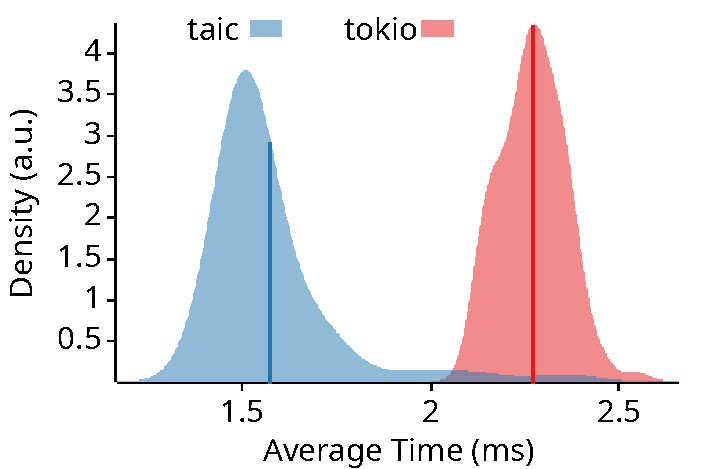
\includegraphics[width=\textwidth]{figures/tokio/chained_spawn.pdf}
		\subcaption{chained\_spawn}
		\label{tokio_chained_spawn}
	\end{minipage}
    \begin{minipage}[c]{0.32\textwidth}
		\centering
		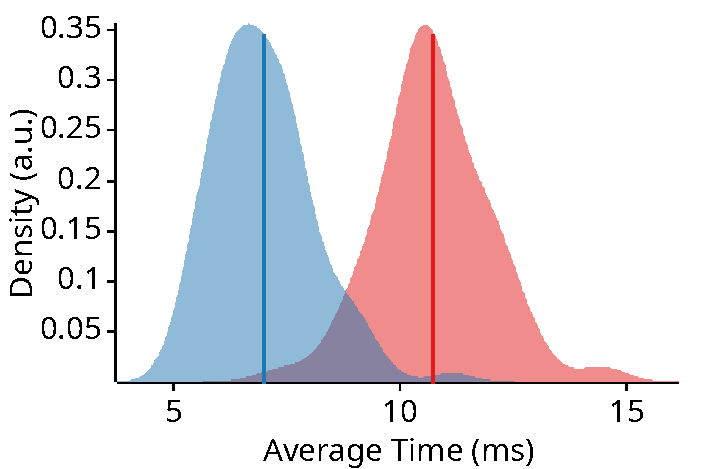
\includegraphics[width=\textwidth]{figures/tokio/spawn_local.pdf}
		\subcaption{spawn\_local}
		\label{tokio_spawn_local}
	\end{minipage}
    \begin{minipage}[c]{0.32\textwidth}
		\centering
		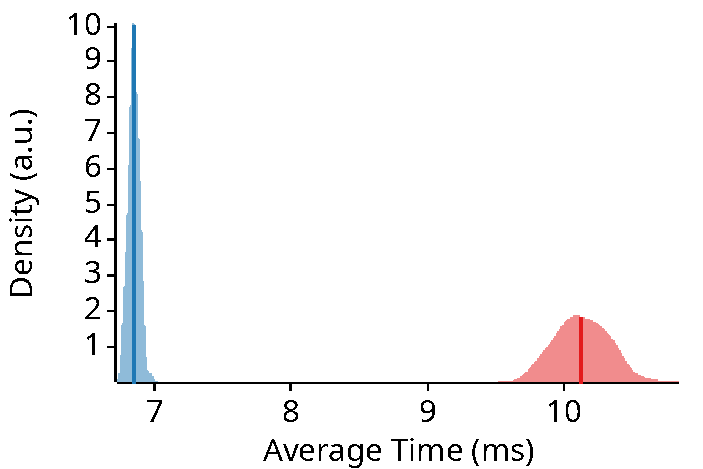
\includegraphics[width=\textwidth]{figures/tokio/spawn_remote_idle.pdf}
		\subcaption{spawn\_remote\_idle}
		\label{tokio_spawn_remote_idle}
	\end{minipage}

    \begin{minipage}[c]{0.32\textwidth}
		\centering
		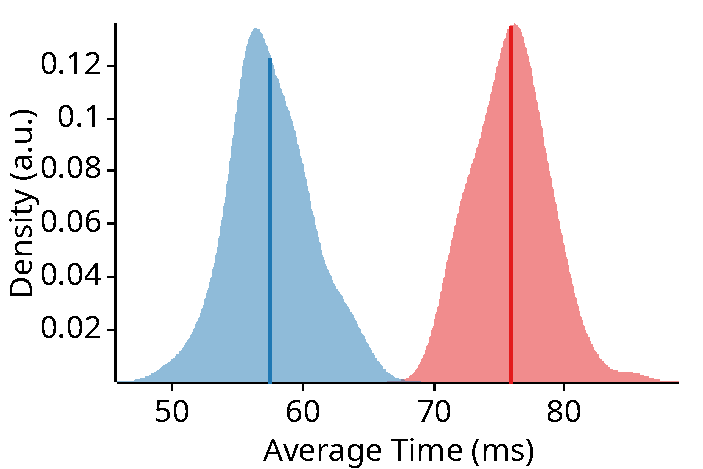
\includegraphics[width=\textwidth]{figures/tokio/yield.pdf}
		\subcaption{yield}
		\label{tokio_yield}
	\end{minipage}
    \begin{minipage}[c]{0.32\textwidth}
		\centering
		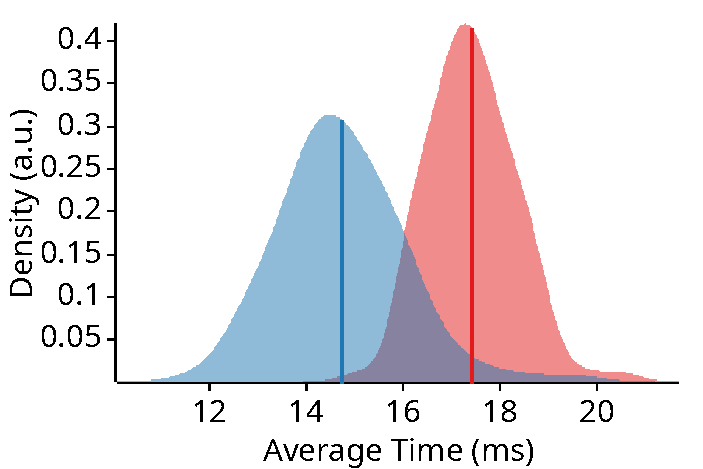
\includegraphics[width=\textwidth]{figures/tokio/ping_pong.pdf}
		\subcaption{ping\_pong}
		\label{tokio_ping_pong}
	\end{minipage}
    \begin{minipage}[c]{0.32\textwidth}
		\centering
		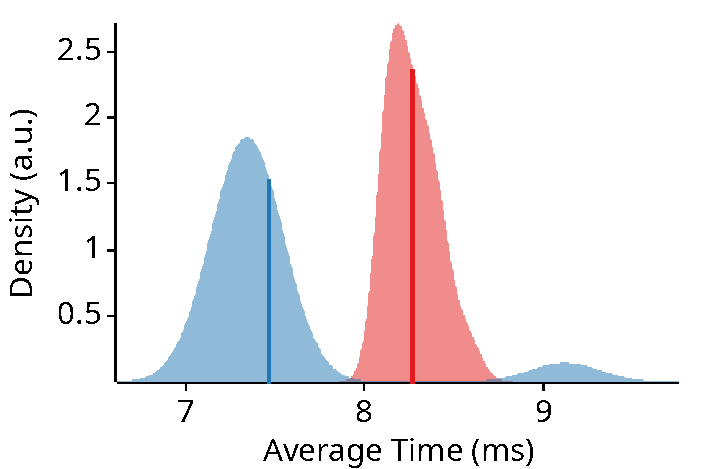
\includegraphics[width=\textwidth]{figures/tokio/spawn_remote_busy.pdf}
		\subcaption{spawn\_remote\_busy}
		\label{tokio_spawn_remote_busy}
	\end{minipage}
    \caption{任务调度对比,其中 taic 表示使用硬件任务队列,tokio 表示使用软件任务队列。}
    \label{figure:tokio-bench}
\end{figure*}

本文对 tokio 默认的多线程调度器进行了修改,将其任务窃取算法中使用的任务队列替换为 TAIC 提供的硬件任务队列。每个工作线程使用 TAIC 提供的硬件局部队列,这些硬件局部队列共同构成一个硬件全局队列,如图 \ref{figure:ready_queue} 所示。由于硬件的局部队列没有固定的容量限制,但其最大容量不超过全局队列的容量,因此修改后的 tokio 任务调度器无法满足规则 \ref{item:push_overflow},为了保证公平,测试过程中保证了不会出现局部队列溢出的情况。此外,由于硬件提供了局部队列之间的负载均衡功能,当局部队列中没有任务时,会自动从其他的局部队列中取出任务,因此,规则 \ref{item:steal_work} 也不再需要,但保留了计算随机数的开销来保证测试的公平性。使用上述修改后的 tokio 调度器来评估 TAIC 在任务调度方面的性能表现,最终的结果如图\ref{figure:tokio-bench}所示。

\textbf{任务窃取}:chained\_spawn 测试递归的生成任务,任意时刻,至多存在两个任务,当一个工作线程运行任务 $A$ 生成一个新的任务 $B$ 时,其他的空闲的工作线程会窃取新生成的任务 $B$ 来执行,循环这个过程,直到结束。因此两个测试的性能差异主要取决于任务窃取的性能。taic 在任务窃取时直接从局部队列中可以窃取出其他的局部队列中的任务,而 tokio 原本的软件任务窃取需要搜索开销以及局部队列的同步互斥等额外开销,从图 \ref{tokio_chained_spawn} 可以看出,taic 使得任务窃取的开销下降了 30.68\%。同理,spawn\_local 测试生成更多的任务,并将任务放入当前工作线程的局部队列中,尽管 tokio 原本的任务窃取会直接从其他局部队列中窃取一半的任务,但 taic 提供的硬件任务窃取功能几乎是零开销的,因此,taic 在 spawn\_local 测试(图\ref{tokio_spawn_local})中仍然将任务窃取的开销下降了 34.88\%。spawn\_remote\_idle 测试(图\ref{tokio_spawn_remote_idle})与 spawn\_local 测试类似,不同之处在于它将生成的任务放到了远端队列(远端队列等价于局部队列,用于任务窃取)中,两者的性能差距仍然来源于任务窃取的开销(32.41\%)。

\textbf{任务切换}:yield(图 \ref{tokio_yield})、ping\_pong(图 \ref{tokio_ping_pong}) 和 spawn\_remote\_busy(图 \ref{tokio_spawn_remote_busy}) 测试了在高频任务切换时,硬件任务队列与软件任务队列的性能差异。在 yield 测试中,每个任务在主动让权若干次后结束;在 ping\_pong 测试中,由于相互发送消息的两个任务需要等待对方的消息;在spawn\_remote\_busy 测试中,用户态任务让权后再次运行时,会使用 \verb|sched_yield| 系统调用让当前的工作线程进入内核态让权。因此,使用 taic 节省的任务窃取开销被分摊到每次任务切换以及等待的过程中,使用 taic 将这三个测试的开销分别降低了 24.22\%、15.37\% 和 9.69\%。其中 spawn\_remote\_busy 测试过程中,因为 Linux 内核产生随机数缓慢,导致了使用 taic 时部分测试的平均延时过高。

\subsection{任务通信}

ipc-bench \cite{ipc-bench_2025} 是一个用于测试 Linux 上的包括信号、管道和 eventfd 等 IPC 机制的开源项目。ipc-bench 针对每种 IPC 机制使用了 ping-pong 通信模型(通信双方忙等对方的消息)来测试其性能,性能指标包括通行的总时间、平均每次通信的时间、吞吐量等。

本文参考 ipc-bench 项目中对信号、管道和 eventfd 等 IPC 机制的测试方法,实现了使用 TAIC 进行任务通信的测试程序。测试程序排除了申请 TAIC 硬件资源以及初始化的时间,测试了通信的总时间。其中,所有测试的消息大小为 1 bit,发送消息次数为 1000 次。各项 IPC 机制的性能对比如图 \ref{figure:ipc-bench} 和表 \ref{tab:ipc-bench} 所示。

\begin{figure}
    \centering
    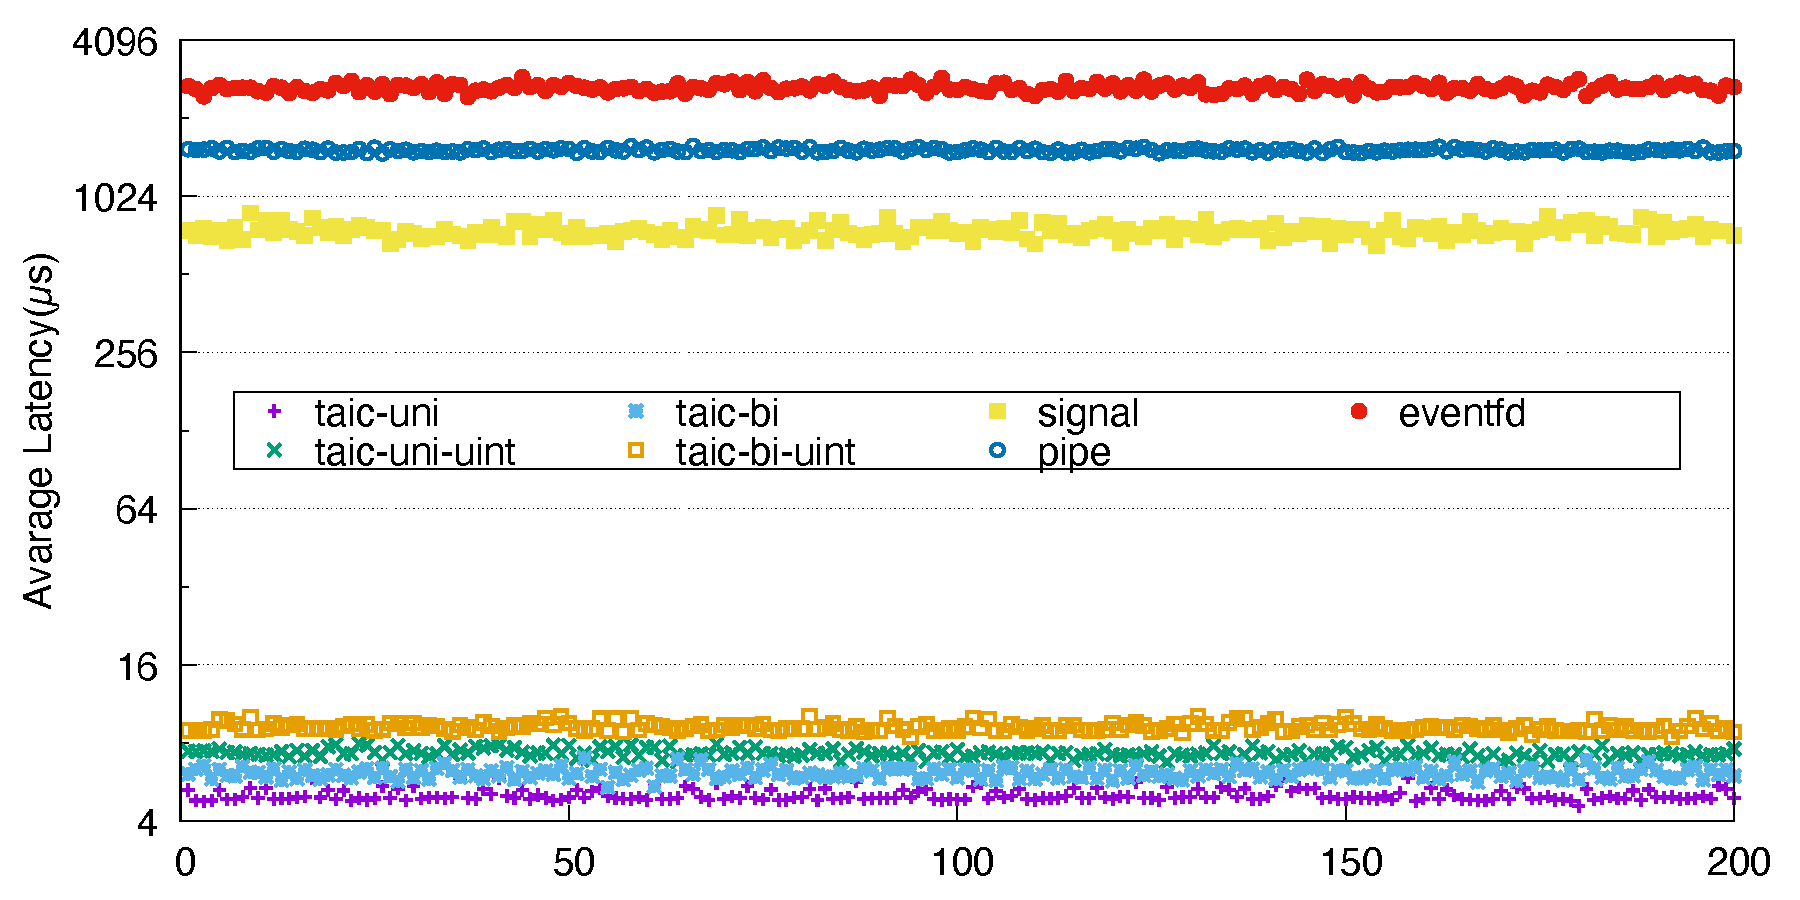
\includegraphics[width=\textwidth]{figures/pdfs/taic-ipc.pdf}
    \caption{IPC 延迟对比,taic 表示使用硬件任务通信机制的测试。其中,bi 表示双向,双方互相发送消息;uni 表示单向;uint 表示任务优先级高,需要发送中断。eventfd、pipe、signal 均为双向;}
    \label{figure:ipc-bench}
\end{figure}

\begin{table}
    \centering
    \caption{IPC 性能对比}
    \label{tab:ipc-bench}
    \begin{tabular}{llll}
        \toprule
        \textbf{测试} & \textbf{吞吐量 $msg/s$} & \textbf{平均延时 $\mu s$} & \textbf{相对延迟比} \\
        \midrule
        taic-uni & 199215.0 & 5.02 & 1 \\
        taic-bi & 163158.4 & 6.13 & 1.221 \\
        taic-uni-uint & 137127.0 & 7.29 & 1.453 \\
        taic-bi-uint & 108734.7 & 9.20 & 1.832 \\
        signal & 1334.7 & 749.23 & 149.258 \\
        pipe & 649.6 & 1539.41 & 306.673 \\
        eventfd & 374.9 & 2667.38 & 531.382 \\
        \bottomrule
    \end{tabular}
\end{table}

与 taic 相关的测试保证了通信的接收方在 CPU 上运行(接收方处于在线状态)。不使用中断时,接收方不断尝试从硬件任务队列中取出被唤醒的任务,一旦取出任务则表示收到通知,结束通信的过程;当使用中断时,接收方收到中断信号后,进入用户态的中断的处理逻辑中,从硬件任务队列中取出被唤醒的任务才算收到通知,但需要从中断返回才结束通信;在双向通信中,接收方收到发送方的通知后,向发送方发起通知,直到发送方收到通知才结束通信的流程。

无论是否使用中断来进行任务抢占,使用 TAIC 进行任务通信的性能都远远优于其他的 IPC 机制,在性能上有数量级的提升,能够达到微秒级的时间尺度。但在不使用中断的情况下,若接收方进程正在执行其他的任务,TAIC 内部的中断处理和中断的开销会被其他任务执行掩盖掉,若其他任务的执行时间也处于微秒级,那么即使不需要中断机制,同样可以达到微秒级的通信延迟。

在 ipc-bench 测试的基础上,本文进一步测试了接收方处于不同的特权级的中断延迟(中断延迟包括了 TAIC 中断处理开销、保存被打断任务上下文开销以及软件进行中断分发的开销)。具体的结果如表 \ref{tab:interrupt-latency}所示,括号内表示不包括 TAIC 中断处理开销的中断延迟。结果证明了使用 TAIC 不会增加中断延迟,保证被唤醒的任务可以及时抢占。

\begin{table}
    \centering
    \caption{中断延迟对比}
    \label{tab:interrupt-latency}
    \begin{tabular}{ll}
        \toprule
        \textbf{接收方特权级} & \textbf{CPU 周期} \\
        \midrule
        用户态 & 72(66) \\
        内核态 & 98(92) \\
        \bottomrule
    \end{tabular}
\end{table}

以上的测试没有包括极端的情况。一种极端的情况是接收方运行于用户态,但接收方的进程没有任务在用户态运行,此时,即使唤醒的任务的优先级较高,也无法进行任务抢占,需要等到接收方的进程中存在任务回到用户态运行时才能进行抢占,此时,任务通信的延时除了用户态中断的开销外,还包括了接收方进程等待被调度的时间以及从内核态返回用户态的开销。另一种极端的情况是接收方运行于内核态,但此时接收方没有任务处于内核态运行,因此任务抢占会导致一个正在运行用户态任务的 CPU 陷入内核态,因此任务通信的开销还会包括特权级切换开销(在本文的实验环境下,开销为 870 个时钟周期)。

\section{综合测试}

\subsection{特征分析}

\section{本章小结}

% 从硬件出发的角度,大多数工作通过设计特殊的硬件或者特殊的指令来绕过内核实现 IPC。如 SkyBridge[11]允许进程在 IPC 中直接切换到目标进程的虚拟地址空间并调用目标函数,它通过精心设计一个虚拟化层(Root Kernel)提供虚拟化的功能,通过 VMFUNC 地址空间的直接切换,并通过其他一系列软件手段来保证安全性,但这种方案仅适用于虚拟化环境中。XPC[12]则直接使用硬件来提供一个无需经过内核的同步功能调用,并提供一种新的空间映射机制用于调用者与被调用者之间的零拷贝消息传递,然而该方案没有相应的硬件标准,也没有一款通用的处理器对其进行支持。这些方法都基于特殊的环境或者没有标准化的硬件来实现,适用范围有限。

% 从软件出发的角度,相关工作主要分为两类:第一类方法通过将用户态和内核态的功能扁平化来减少内核与用户态的切换开销,如 unikernel[13, 14, 15]将所有用户态代码都映射到内核态执行,Userspace Bypass[16]通过动态二进制分析将两个系统调用之间的用户态代码移入内核态执行,从而减少陷入内核的次数,kernel bypass[17, 18]则通过将硬件驱动(传统内核的功能)移入用户态,从而减少上下文的切换。这些方法要么需要特殊的硬件支持,要么难以与微内核的设计理念兼容。第二类方法则是允许用户空间对多个系统调用请求排队,并通过一次提交将他们注册给内核,如 FlexSC[19]通过在用户态设计一个用户态线程的运行时,将用户态线程发起的系统调用自动收集,然后陷入内核态进行批量执行。该方法虽然可以有效的减少陷入内核的次数,但如何设置提交的时机难以把握,过短的提交间隔将导致切换次数增加,过长的提交间隔则会导致 CPU 空转。

% 虽然现有工作难以广泛且有效地应用到微内核中,但他们的思路值得我们借鉴,他们的缺陷驱使我们去寻求更好的方案。在硬件方面,一种新型的硬件技术方案——用户态中断[20, 21]逐渐被各个硬件平台(x86,RISC-V)采纳,它通过在 CPU 中新增中断代理机制和用户态中断的状态寄存器,当中断代理机制检测到状态寄存器发生变化时,会将中断以硬件转发的形式传递给用户态程序,从而绕过内核。该硬件方案已经在 Sapphire Rapids x86 处理器上和 RISCV 的 N 扩展中有了一定的支持,适用范围更加广泛。而在软件方面,异步被广泛用于请求合并和开销均摊,传统类 Unix 系统提供的类似 select IO 多路复用接口相对简陋,迫使用户态代码采用事件分发的编程范式来处理异步事件,代码相对复杂,可读性较弱。而新兴的 Rust[22, 23]语言对异步有着良好的支持,其零成本抽象的设计也让它作为系统编程语言有着强大的竞争力。使用 Rust 进行内核和用户态基础库的开发,可以更好地对异步接口进行抽象,改善接口的易用性和代码的可读性。

% 我们在FPGA平台上对TAIC进行了一系列评估,旨在解决几个核心问题:

% 上下文切换的影响:我们首先评估了TAIC的快速唤醒机制相对于传统中断机制的性能优势,以了解其性能益处的来源。

% CPU利用率的影响:其次,我们检查了TAIC的快速唤醒机制对CPU利用率的影响。理解这一点对于评估TAIC在提高CPU利用率和降低CPU负载方面的有效性至关重要。

% 优先队列对I/O请求处理的影响:我们还研究了TAIC内部的优先队列如何影响不同优先级的I/O请求处理。这有助于我们理解TAIC在处理复杂I/O工作负载时的性能特点。

% 实际应用中的性能改进:最后,我们探讨了TAIC在实际应用场景中提供的延迟和吞吐量的改进程度。这项评估将为我们提供TAIC在现实条件下的性能数据,使我们能够评估其对整体系统性能的贡献。

% 通过这些评估,我们希望全面了解TAIC的性能特点,并为未来的优化和应用提供实证基础。

% 实验设置

% 为了评估TAIC的性能,我们选择了Xilinx的Zynq UltraScale+ XCZU15EG-2FFVB1156 MPSoC作为我们的FPGA平台。这款高性能的系统级芯片(SoC)为我们提供了充足的资源来实现复杂的硬件加速任务。我们的工作基于Rocket-chip项目[3],这是一个开源的RISC-V架构,五级流水线处理器软核(四核,100MHz)。利用这个基础,我们实现了TAIC中断控制器,以利用其快速唤醒功能机制。此外,我们构建了一个高效的异步网络卡驱动程序,专门设计用于处理网络I/O请求。我们选择了Xilinx AXI 1G/2.5G以太网子系统(1Gbps)作为我们的网络接口,并配备了Xilinx AXI DMA控制器以促进高速数据传输。

% 异步 IPC 作为 ReL4 中的主要的 IPC 方式,其实现依赖于异步运行时和 U-notification。我们以 IPC 中最常见的 Call为例,客户端进程和服务端进程在双方建立连接时都会注册一个 dispatcher 协程用于不断从共享缓冲区中读取数据并进行处理。我们分别对服务端和客户端的 dispatcher 协程提供了两个默认实现,对于特殊的需求,用户程序可以通过运行时接口自定义 dispatcher 协程的行为。服务端的 dispatcher协程读取请求并处理后将响应写入环形缓冲区,并根据标志位判断是否发送 U-notification,没有请求时阻塞自己并切换到其他 worker 协程。客户端的 dispatcher 协程读取响应并唤醒响应的协程,没有响应时阻塞切换。Call 的主要流程分为以下几个阶段:

% 1)客户端发起请求:用户态程序将以 worker 协程的形式发起 IPC 请求,异步运行时首先会根据请求的数据和协程的协程号生成 IPCItem 并写入请求的环形缓冲区中并将当前协程阻塞,然后检查缓冲区的 req\_co\_status 标志位,如果对方的 dispatcher 协程已经就绪,那我们无需通知对方进程,对方进程的异步运行时会在某个时刻调度到 dispatcher协程并处理请求。如果对方的 dispatcher 协程处于阻塞状态,则异步运行时会将 req\_co\_status 标志位置位,并发送 Unotification 通知对方进程唤醒 dispatcher 协程并重启调度。

% 2)服务端处理请求并写回响应:服务端的 dispatcher 协程会在合适的时机读取出请求并进行解码和处理,然后根据处理结果构造响应的 IPCItem 并写入响应的环形缓冲区中,检查缓冲区中的 reply\_co\_status 标志位,如果客户端的响应 dispatcher 协程就绪,则无需发起通知,否则需要发起 Unotification 通知客户端进程唤醒 dispatcher 协程并重启调度。如果缓冲区内容为空,dispatcher 协程会将 req\_co\_status 标志位置空,并将自己阻塞。

% 3)客户端处理响应:客户端的 dispatcher 协程会在合适的时机读取响应并唤醒之前阻塞的协程,然后重启调度。

% 从广义的角度来看,异步系统调用是一类特殊的异步IPC,其接收方为内核。因此我们在内核中提供了一套相似的异步运行时以支持异步系统调用。异步系统调用与异步IPC 的主要不同之处有两点:

% 1) 由于接收端是内核,发送端无法使用 U-notification 去通知内核。

% 2) 异步 IPC 中进程的异步调度器就是进程的执行主体,无需考虑异步任务的执行时机,而内核除了异步系统调用请求需要调度器执行,本身就有如中断、异常、任务调度等其他任务需要被执行。对于第一点,我们只需要新增一个系统调用去用于唤醒相关的内核协程即可。而对于第二点,一个很简单的思路是每次时钟中断到来时去执行异步系统调用,然而这可能会导致空闲的 CPU 核心无法及时触发时钟中断而空转,因此,在不破坏原本的线程优先级调度前提下,我们使用核间中断来抢占空闲 CPU 核心或正在运行低优先级线程的 CPU 核心,更好地利用空闲 CPU 资源,减少响应时延。为了避免破坏微内核中原本的优先级调度机制,我们在内核中对 每 个 CPU 核心维护了相应的执行优先级(exec\_prio),执行优先级区别于上文提到的运行时协程优先级,是由内核调度器维护的线程优先级。内核中的任务主要分为三类:1) idle\_thread: 空闲 CPU 核心执行 idle 线程,此时 CPU 核心的执行优先级为 256,属于最低的执行优先级。2) 内核态任务:正在处理中断、异常、系统调用等,此时CPU 核心的执行优先级为 0,最高优先级,不可被抢占。3) 用户态任务:正在执行用户态的任务,此时 CPU 核心的执行优先级为当前线程的优先级,可以被更高优先级线程提交的异步系统调用请求打断。

% 当发送端通过系统调用陷入内核去唤醒相应协程后,会检查当前线程的优先级是否可以抢占其他 CPU 核心,如果可以,则发送核间中断抢占该 CPU 核心去执行异步系统调用,当前 CPU 核心则返回用户态继续执行其他协程。如果没有可以被抢占的 CPU 核心,则在下一次时钟中断到来时执行异步系统调用请求,其伪代码如下:

% 为了从微观角度评估我们设计的异步 IPC 性能,我们测量了不同并发量和不同服务端负载下异步 IPC 和同步 IPC的平均开销。由于我们关注的是同步 IPC 和异步 IPC 的路径差异,需要保证场景没有过多干扰,因此我们分别构建了一个服务端进程和一个客户端进程进行乒乓测试,测试结果如图 5 所示。

% 由于同步 IPC 会阻塞整个线程,因此并发量对同步 IPC并没有意义。而在多核环境下,fast-path 检查会失败,所有的同步 IPC 都会在内核中通过核间中断进行传递,因此多核环境下的同步 IPC 性能很低;而对于单核下的同步 IPC,fast-path 会避开复杂的消息解码和冗长的调度流程,因此开启fast-path的IPC性能会提升167\%,但我们需要注意的是,fast-path 对于线程优先级、消息长度等有着严苛的检查流程,因此在实际应用场景中 fast-path 优化并不总能生效。

% 我们从横向的角度分析异步 IPC,发现异步 IPC 的开销随着并发量的提升而降低,这是由于随着并发量的增加,服务端的负载进一步增加,而 U-notification 的通知时机采用自适应的形式,因此通知频率下降,导致了均摊到每个 IPC的开销下降。我们还可以看出,在并发度较小的时候,多核会略快于单核(最高提升 52\%),符合预期,随着并发度的逐渐增加,多核与单核的性能差异逐渐缩小(17\%),这是由于多核情况下服务端单独使用一个 CPU 核心,导致服务端负载过小,产生了更加频繁的用户态中断(如左图中的蓝色折线),导致服务端吞吐量过小,又反过来限制了客户端的请求频率。可以从第二幅图中看出,当我们增加服务端负载时,服务端的中断频率会逐渐下降,直至归 0,这是自适应轮询带来的优势。

% 对比同步 IPC 和异步 IPC,当并发度为 1 的时候,每个异步 IPC 的开销都包含了两次用户态中断的开销、调度器的运行时开销,而同步 IPC 则是两次特权级切换的开销,如果没有 fast-path 优化,还会有内核路径中的解码开销和调度开销,因此在低并发度的场景下异步 IPC 的性能会略低于没有fast-path 优化的同步 IPC(31\%),同时显著低于有 fast-path优化的同步 IPC(249\%)。而当并发量较大时,用户态中断的频率减少,均摊到每一次 IPC 下,用户态中断的开销几乎可以忽略不计,因此异步 IPC 的开销主要是调度器的运行时开销,而此时的异步 IPC 性能会显著高于没有 fast-path 优化的同步 IPC(369\%),也高于有 fast-path 优化的同步 IPC(76\%)。

% 从上面我们可以得出结论:在多核场景下,我们的异步IPC 相比于同步始终有着良好的表现。而在单核且低并发度场景下,异步 IPC 性能会比较差,但随着并发度增加,异步IPC 的性能会迅速提升,在并发度为 2 时就已经超过没有fast-path 优化的同步 IPC,在并发度为 8 时就已经超过了开启 fast-path 优化的同步 IPC,因此异步 IPC 依然十分有竞争力。

% 为了测试异步 IPC 在真实应用场景带来的收益,我们在ReL4 上实现了一个 TCP 服务器。模拟的 TCP 服务器应用场景由三部分组成,一部分是运行在 PC 上的客户端,它在启动时与运行在 FPGA 上的 TCP Server 建立若干个连接,并不断地向服务端发送 64 字节(小包)的数据,并接收服务器的响应;第二部分是运行在 ReL4 上的网络协议栈服务器(NW Stack Server),集成了网卡驱动的代码,并通过smoltcp 协议栈维护每个连接的状态信息,负责从网卡中接收数据并进行协议处理后通过共享缓冲区返回给 TCP Server,以及从 TCP Server 接收数据并通过网卡发出;第三部分是 TCP Server,它以 IPC 的形式从 NW Stack Server 接收客户端发送过来的请求,在处理完成之后返回响应并通过NW Stack Server 发送给客户端。最后,PC 上的客户端计算发送每个请求和接收响应之间的时间延迟,并计算固定时间段内的消息吞吐量。我们通过分析不同配置下 TCP Server 的时间延迟和吞吐量来评估 ReL4。需要注意的是,由于同步 IPC 的无法支持多路复用,因此同步 IPC 下每个连接都使用单独的线程来监听。测试结果如图 6 所示。

% 从总体趋势上看,吞吐量随着并发度的增加呈现先增加后减少的趋势,而时延成整体上升的趋势。在低并发度条件下的系统负载处于较低水平,随着并发度增加,吞吐量能稳步提升,随着系统满载之后,继续增加并发度,会导致网络中断频率上升,从而限制系统的整体性能,吞吐量减少。

% 同步和异步对比来看,可以看出当连接数较低,并发度较小的情况下,异步 IPC 实现的 TCP Server 无论是在吞吐率还是平均时延上都要优于同步 IPC,这是由于同步 IPC 需要频繁陷入内核,而由于微内核不可被抢占的设计,内核态屏蔽了网络中断,导致网络包无法及时处理。而随着并发度的增加,由于同步 IPC 实现的 TCP Server 需要多线程来保证多连接,因此线程切换的开销急剧加大,导致同步和异步的差距进一步增加。在连接数为 4 的时候差距达到最大,为192\%,在并发度最大的情况下,异步 IPC 实现的 TCP Server也比同步 IPC 高出 120\%。

% 单核与多核对比来看,异步 IPC 实现的 TCP Server 随着 CPU 资源增加,吞吐量提升,时延降低,而对于同步 IPC实现的 TCP Server 情况则有所不同,由于同步 IPC 在多核下采用的 IPI 的形式在内核进行转发,导致程序的内存局部性和代码局部性都不够友好,因此多核的性能变现会略低于单核。

% 从上面我们可以得出结论:异步 IPC 在实际应用场景中有利于多路复用的实现,可以有效减少特权级切换的开销,提升系统的整体性能。

\chapter{总结与展望}

本文在总结现有研究工作的基础上,提出了基于执行流的任务模型,

% 挑战
% 空间容量的挑战:目前,TAIC内部实现的队列正面临空间容量方面的挑战。随着队列长度的增加,所需的硬件资源也在增长。在实际应用场景中,可能需要处理成千上万的任务,这使得TAIC有限的内部空间容量难以满足如此庞大的请求数量。

% 为了解决这个问题,我们提出了一种新的设计,但尚未实施:在内存中维护就绪队列和阻塞槽,但确保它们只被TAIC访问,并向TAIC添加一个数据迁移组件。相应地调整TAIC的中断处理功能——数据迁移组件将阻塞任务的标识符从内存中的阻塞槽移动到内存中的就绪队列。这种方法旨在解决硬件空间容量问题,我们计划在后续工作中推进这一设计。

% 对延迟的影响:尽管TAIC能够处理中断并及时唤醒被阻塞的任务,但这并不能保证唤醒的任务可以立即执行。当当前CPU忙于处理其他具有更高优先级的任务时,这种情况可能会发生。如果有恶意任务(例如,可能由于紧密循环而不断占用CPU的任务),它们可能会独占CPU资源,导致系统延迟增加。在这些情况下,我们认为这些任务的行为是不适当的,因为它们没有与其他任务适当合作和共享资源。为了减少这种不良行为对系统延迟的影响,我们可以使用工具和机制来监控和限制任务的CPU使用。例如,编译器可以强制执行合作政策,确保任务在执行一定时间后将CPU让给其他任务(就像Concord[29]一样)。此外,运行时分析工具可以用来检测和识别长时间占用CPU的任务,以便进行调整或优化。此外,适当的优先级设置可以确保及时响应。

% 展望

% 使用场景:目前,我们仅在单核环境中使用TAIC。然而,TAIC在使用场景的选择上具有一定的灵活性。它不受CPU特权级别的限制,允许在用户空间使用。这使得用户进程能够通过将TAIC的地址空间映射到自己的空间中,构建高效的用户空间异步设备驱动程序。这种方法避免了传统内核旁路技术中检查设备状态的低效轮询方法,从而提高了性能。(与在用户空间使用uintr[2]相比,不同的路径通往同一个目标。)然而,当前的设计限制是TAIC在任何给定时刻只能被单个进程使用。当多个进程需要同时使用TAIC时,需要在内核中实现更严格的控制机制,以防止潜在的冲突和不可预测的行为。为了解决这个问题,我们计划在未来的研发中进一步完善设计,以支持多个进程安全高效地共享TAIC资源。

% 可扩展性:不仅外设,软件和定时器也可以是中断源。TAIC可以设计成允许软件通过写入相应的接口来触发软件中断。软中断在操作系统中扮演着重要角色,通常用于处理系统调用、进程间同步以及进程间通信(IPC)。如果使用TAIC来加速软中断的处理,不仅可以加快系统调用的响应速度,还可以提高IPC的效率。我们期望通过这些研究进一步提高系统的整体性能,特别是在高负载场景下,频繁的系统调用和IPC是必需的。此外,定时器中断作为操作系统调度机制的关键组成部分,直接影响操作系统的响应性和实时性能。因为内核调度器被卸载到TAIC中,所以在TAIC内处理定时器中断是可能的,这可以进一步优化操作系统的调度性能。探索TAIC在处理定时器中断中的应用将是我们未来研究的一个重要方向。我们期待通过这些研究更全面地增强系统的中断处理能力,从而为构建高效可靠的操作系统提供坚实的基础。

% TAIC,从内核中卸载了调度器的功能,是一个具有任务感知和任务调度能力的中断控制器。TAIC解决了CPU与I/O设备交互中的信息不对称问题。TAIC可以在中断处理例程中,不通过CPU从中断控制器获取信息,而是从其内部结构中获取中断相关信息,从而避免了CPU上下文切换的开销,并消除了CPU维护调度队列的需要。使用FPGA进行的评估表明,TAIC可以减少由中断引起的上下文切换开销,优化CPU利用率,并提高系统吞吐量。



% 其他部分
\backmatter

% 参考文献
\bibliography{ref/refs}  % 参考文献使用 BibTeX 编译
% \printbibliography       % 参考文献使用 BibLaTeX 编译

% 附录
% 本科生需要将附录放到声明之后,个人简历之前
\appendix
% % !TeX root = ../thuthesis-example.tex

\begin{survey}
\label{cha:survey}

\title{Title of the Survey}
\maketitle


\tableofcontents


本科生的外文资料调研阅读报告。


\section{Figures and Tables}

\subsection{Figures}

An example figure in appendix (Figure~\ref{fig:appendix-survey-figure}).

\begin{figure}
  \centering
  
\includegraphics[width=0.6\linewidth]{example-image-a.pdf}
  \caption{Example figure in appendix}
  \label{fig:appendix-survey-figure}
\end{figure}


\subsection{Tables}

An example table in appendix (Table~\ref{tab:appendix-survey-table}).

\begin{table}
  \centering
  \caption{Example table in appendix}
  \begin{tabular}{ll}
    \toprule
    File name       & Description                                         \\
    \midrule
    thuthesis.dtx   & The source file including documentation and comments \\
    thuthesis.cls   & The template file                                   \\
    thuthesis-*.bst & BibTeX styles                                       \\
    thuthesis-*.bbx & BibLaTeX styles for bibliographies                  \\
    thuthesis-*.cbx & BibLaTeX styles for citations                       \\
    \bottomrule
  \end{tabular}
  \label{tab:appendix-survey-table}
\end{table}


\section{Equations}

An example equation in appendix (Equation~\eqref{eq:appendix-survey-equation}).
\begin{equation}
  \frac{1}{2 \uppi \symup{i}} \int_\gamma f = \sum_{k=1}^m n(\gamma; a_k) \mathscr{R}(f; a_k)
  \label{eq:appendix-survey-equation}
\end{equation}


\section{Citations}

Example\cite{dupont1974bone} citations\cite{merkt1995rotational} in appendix
\cite{dupont1974bone,merkt1995rotational}.


% 默认使用正文的参考文献样式;
% 如果使用 BibTeX,可以切换为其他兼容 natbib 的 BibTeX 样式。
\bibliographystyle{unsrtnat}
% \bibliographystyle{IEEEtranN}

% 默认使用正文的参考文献 .bib 数据库;
% 如果使用 BibTeX,可以改为指定数据库,如 \bibliography{ref/refs}。
\printbibliography

\end{survey}
       % 本科生:外文资料的调研阅读报告
% % !TeX root = ../thuthesis-example.tex

\begin{translation}
\label{cha:translation}

\title{书面翻译题目}
\maketitle

\tableofcontents


本科生的外文资料书面翻译。


\section{图表示例}

\subsection{图}

附录中的图片示例(图~\ref{fig:appendix-translation-figure})。

\begin{figure}
  \centering
  
\includegraphics[width=0.6\linewidth]{example-image-a.pdf}
  \caption{附录中的图片示例}
  \label{fig:appendix-translation-figure}
\end{figure}


\subsection{表格}

附录中的表格示例(表~\ref{tab:appendix-translation-table})。

\begin{table}
  \centering
  \caption{附录中的表格示例}
  \begin{tabular}{ll}
    \toprule
    文件名          & 描述                         \\
    \midrule
    thuthesis.dtx   & 模板的源文件,包括文档和注释 \\
    thuthesis.cls   & 模板文件                     \\
    thuthesis-*.bst & BibTeX 参考文献表样式文件    \\
    thuthesis-*.bbx & BibLaTeX 参考文献表样式文件  \\
    thuthesis-*.cbx & BibLaTeX 引用样式文件        \\
    \bottomrule
  \end{tabular}
  \label{tab:appendix-translation-table}
\end{table}


\section{数学公式}

附录中的数学公式示例(公式\eqref{eq:appendix-translation-equation})。
\begin{equation}
  \frac{1}{2 \uppi \symup{i}} \int_\gamma f = \sum_{k=1}^m n(\gamma; a_k) \mathscr{R}(f; a_k)
  \label{eq:appendix-translation-equation}
\end{equation}


\section{文献引用}

附录\cite{dupont1974bone}中的参考文献引用\cite{merkt1995rotational}示例
\cite{dupont1974bone,merkt1995rotational}。


\appendix

\section{附录}

附录的内容。


% 书面翻译的参考文献
% 默认使用正文的参考文献样式;
% 如果使用 BibTeX,可以切换为其他兼容 natbib 的 BibTeX 样式。
\bibliographystyle{unsrtnat}
% \bibliographystyle{IEEEtranN}

% 默认使用正文的参考文献 .bib 数据库;
% 如果使用 BibTeX,可以改为指定数据库,如 \bibliography{ref/refs}。
\printbibliography

% 书面翻译对应的原文索引
\begin{translation-index}
  \nocite{mellinger1996laser}
  \nocite{bixon1996dynamics}
  \nocite{carlson1981two}
  \bibliographystyle{unsrtnat}
  \printbibliography
\end{translation-index}

\end{translation}
  % 本科生:外文资料的书面翻译
% % !TeX root = ../thuthesis-example.tex

\chapter{补充内容}

附录是与论文内容密切相关、但编入正文又影响整篇论文编排的条理和逻辑性的资料,例如某些重要的数据表格、计算程序、统计表等,是论文主体的补充内容,可根据需要设置。

附录中的图、表、数学表达式、参考文献等另行编序号,与正文分开,一律用阿拉伯数字编码,
但在数码前冠以附录的序号,例如“图~\ref{fig:appendix-figure}”,
“表~\ref{tab:appendix-table}”,“式\eqref{eq:appendix-equation}”等。


\section{插图}

% 附录中的插图示例(图~\ref{fig:appendix-figure})。

\begin{figure}
  \centering
  
\includegraphics[width=0.6\linewidth]{example-image-a.pdf}
  \caption{附录中的图片示例}
  \label{fig:appendix-figure}
\end{figure}


\section{表格}

% 附录中的表格示例(表~\ref{tab:appendix-table})。

\begin{table}
  \centering
  \caption{附录中的表格示例}
  \begin{tabular}{ll}
    \toprule
    文件名          & 描述                         \\
    \midrule
    thuthesis.dtx   & 模板的源文件,包括文档和注释 \\
    thuthesis.cls   & 模板文件                     \\
    thuthesis-*.bst & BibTeX 参考文献表样式文件    \\
    thuthesis-*.bbx & BibLaTeX 参考文献表样式文件  \\
    thuthesis-*.cbx & BibLaTeX 引用样式文件        \\
    \bottomrule
  \end{tabular}
  \label{tab:appendix-table}
\end{table}


\section{数学表达式}

% 附录中的数学表达式示例(式\eqref{eq:appendix-equation})。
\begin{equation}
  \frac{1}{2 \uppi \symup{i}} \int_\gamma f = \sum_{k=1}^m n(\gamma; a_k) \mathscr{R}(f; a_k)
  \label{eq:appendix-equation}
\end{equation}


\section{文献引用}

附录\cite{dupont1974bone}中的参考文献引用\cite{zhengkaiqing1987}示例
\cite{dupont1974bone,zhengkaiqing1987}。

\printbibliography


% 致谢
% !TeX root = ../thuthesis-example.tex

\begin{acknowledgements}
  衷心感谢导师×××教授和物理系××副教授对本人的精心指导。他们的言传身教将使我终生受益。

  在美国麻省理工学院化学系进行九个月的合作研究期间,承蒙 Robert Field 教授热心指导与帮助,不胜感激。

  感谢×××××实验室主任×××教授,以及实验室全体老师和同窗们学的热情帮助和支持!

  本课题承蒙国家自然科学基金资助,特此致谢。
\end{acknowledgements}


% 声明
% 本科生开题报告不需要
\statement
% 将签字扫描后的声明文件 scan-statement.pdf 替换原始页面
% \statement[file=scan-statement.pdf]
% 本科生编译生成的声明页默认不加页脚,插入扫描版时再补上;
% 研究生编译生成时有页眉页脚,插入扫描版时不再重复。
% 也可以手动控制是否加页眉页脚
% \statement[page-style=empty]
% \statement[file=scan-statement.pdf, page-style=plain]

% 个人简历、在学期间完成的相关学术成果
% 本科生可以附个人简历,也可以不附个人简历
% !TeX root = ../thuthesis-example.tex

\begin{resume}

  \section*{个人简历}

  197× 年 ×× 月 ×× 日出生于四川××县。

  1992 年 9 月考入××大学化学系××化学专业,1996 年 7 月本科毕业并获得理学学士学位。

  1996 年 9 月免试进入清华大学化学系攻读××化学博士至今。


  \section*{在学期间完成的相关学术成果}

  \subsection*{学术论文}

  \begin{achievements}
    \item Yang Y, Ren T L, Zhang L T, et al. Miniature microphone with silicon-based ferroelectric thin films[J]. Integrated Ferroelectrics, 2003, 52:229-235.
    \item 杨轶, 张宁欣, 任天令, 等. 硅基铁电微声学器件中薄膜残余应力的研究[J]. 中国机械工程, 2005, 16(14):1289-1291.
    \item 杨轶, 张宁欣, 任天令, 等. 集成铁电器件中的关键工艺研究[J]. 仪器仪表学报, 2003, 24(S4):192-193.
    \item Yang Y, Ren T L, Zhu Y P, et al. PMUTs for handwriting recognition. In press[J]. (已被Integrated Ferroelectrics录用)
  \end{achievements}


  \subsection*{专利}

  \begin{achievements}
    \item 任天令, 杨轶, 朱一平, 等. 硅基铁电微声学传感器畴极化区域控制和电极连接的方法: 中国, CN1602118A[P]. 2005-03-30.
    \item Ren T L, Yang Y, Zhu Y P, et al. Piezoelectric micro acoustic sensor based on ferroelectric materials: USA, No.11/215, 102[P]. (美国发明专利申请号.)
  \end{achievements}

\end{resume}


% 指导教师/指导小组评语
% 本科生不需要
% !TeX root = ../thuthesis-example.tex

\begin{comments}
% \begin{comments}[name = {指导小组评语}]
% \begin{comments}[name = {Comments from Thesis Supervisor}]
% \begin{comments}[name = {Comments from Thesis Supervision Committee}]

  论文提出了……

\end{comments}


% 答辩委员会决议书
% 本科生不需要
% !TeX root = ../thuthesis-example.tex

\begin{resolution}

  论文提出了……

  论文取得的主要创新性成果包括:

  1. ……

  2. ……

  3. ……

  论文工作表明作者在×××××具有×××××知识,具有××××能力,论文××××,答辩××××。

  答辩委员会表决,(×票/一致)同意通过论文答辩,并建议授予×××(姓名)×××(门类)学博士/硕士学位。

\end{resolution}


% 本科生的综合论文训练记录表(扫描版)
% \record{file=scan-record.pdf}

\end{document}
